\subsection[补充]{补充\footnote{在本号中，我们使用了《交换代数》一书中尚在编写中的各章的结果，并用“交换代数”这一名称来标示它们。}}

引理 4. 设 K 是交换域，V 是 K 上的有限维向量空间，G 是由 V 的自同构组成的有限群，其阶 q 在 K 中可逆，S 是 V 的对称代数，R 是 S 中由在 G 下不变的元素组成的子代数。S 的高度为 1 的素理想 B 在 \(p = B \cap R\) 上分歧（Commutative Algebra）当且仅当存在 V 的非零元素 a 与 \(V^{*}\) 的非零元素 f，使得 B = Sa 且伪反射 \(s_{a,f}\) 属于 G。此时，分解群 \(\mathcal{G}^{\mathrm{Z}}(\mathrm{B})\) 是 G 中使 Ka 稳定的元素所成的子群，惯性群 \(\mathcal{G}^{\mathrm{T}}(\mathrm{B})\) 是 G 的循环子群 \(H_{a}\)，由 G 中以 a 为向量的诸伪反射组成。S 在 B 处的剩余域 S(B) 在 R 于 p 处的剩余域 R(p) 上是可分的，而分歧指数 \(e(\mathrm{B}/\mathfrak{p})\) ——即 B 在差积的除子 \(\text{div}(D_{S/R})\) 中的系数再加 1——等于 \(\text{Card}(H_{a})\)。

说 B 在 R 上分歧，就是指其惯性群 \(\mathcal{G}^{\mathrm{T}}(\mathrm{B})\) 不化为单位元群，换言之，存在 G 中的 \(g \neq 1\)，使得 \(g(z) \equiv z \pmod{B}\) 对所有 \(z \in S\) 都成立。由于 S 是唯一分解环，B 是主理想 Sa，且 a 必须整除所有元素 \(g(z) - z\)（\(z \in S\)）；而当 \(z \in V\) 时，这些元素都是 1 次齐次的，并且都非零（因为 \(g \neq 1\)）；因此 a 必是 1 次齐次的，换言之 \(a \in V\)。于是存在 V 上的线性型 f，使得 \(g = s_{a,f}\)。反之，若 g 是异于 1 的伪反射 \(s_{a,f}\)，则 \(g(z) \equiv z \pmod{Sa}\) 对所有 \(z \in S\) 都成立，故 g 属于素理想 B = Sa 的惯性群。这就证明了引理的第一个断言，以及 \(\mathcal{G}^{\mathrm{Z}}(\mathrm{B})\) 与 \(\mathcal{G}^{\mathrm{T}}(\mathrm{B})\) 的特征刻画。由于 q 与 K 的特征 p 互素（该特征也是 S(B) 的特征），R(p) 的扩张 S(B) 是可分的（Commutative Algebra, Chap. V, §2, no. 2, Cor. of Prop. 5）。由此即得等式 \(e(\mathrm{B}/\mathfrak{p}) = \mathrm{Card}(\mathrm{H}_{a})\)（Commutative Algebra）。由于 \(e(\mathrm{B}/\mathfrak{p})\) 与 p 互素，B 在 \(\operatorname{div}(\mathrm{D}_{\mathrm{S/R}})\) 中的系数为 \(e(\mathrm{B}/\mathfrak{p}) - 1\)（Commutative Algebra）。引理得证。

引理 5. 设 K 是交换域，S 是 K 上的分次多项式代数，R 是 S 的分次子代数。则 S 是自由分次 R-模（Algebra, Chap. II, §11, no. 2）当且仅当下列两个条件得到满足：a) R 是 K 上的分次多项式代数；

\begin{enumerate}
\def\labelenumi{\alph{enumi})}
\setcounter{enumi}{1}
\tightlist
\item
  若 \((\alpha_{1},\ldots,\alpha_{s})\) 是 K-代数 R 的一个由代数无关的齐次元素组成的生成元组，则该组是一个 S-正则序列 \(^{5}\)。
\end{enumerate}

当 S 是有限型 R-模时，b) 是 a) 的推论。

证明见 Commutative Algebra。

定理 4. 设 K 是交换域，V 是 K 上的有限维向量空间，S 是 V 的对称代数，G 是由 V 的自同构组成的有限群，R 是 S 中由在 G 下不变的元素组成的子代数。假设 q = Card G 在 K 中可逆。则下列条件等价：

\begin{enumerate}
\def\labelenumi{(\roman{enumi})}
\item
  G 由伪反射生成；
\item
  S 是自由分次 R-模；
\item
  \(\mathbf{R}\) 是 \(\mathbf{K}\) 上的分次多项式代数。
\end{enumerate}

(ii) 与 (iii) 的等价性由第 2 号及引理 5 得出。蕴涵关系 (i) \(\Longrightarrow\) (ii) 由 Th. 1 得出。

我们证明 (iii) \(\Longrightarrow\) (i)。设 \(G'\) 是 \(G\) 中由属于 \(G\) 的伪反射生成的子群，\(R'\) 是 \(S\) 中由在 \(G'\) 下不变的元素组成的子代数。我们有 \(R \subset R' \subset S\)。由引理 4，\(\text{div}(D_{S/R}) = \text{div}(D_{S/R'})\)，故 \(\text{div}(D_{R'/R}) = 0\)。于是设 \(R\) 是分次多项式代数。由于 \(R'\) 也是如此（因为 \(G'\) 由伪反射生成），引理 5 表明 \(R\)-模 \(R'\) 具有齐次基 \((Q_1, \ldots, Q_m)\)；设 \(q_i = \deg(Q_i)\)。置

\[
d = \det (\mathrm{Tr} _ {R ^ {\prime} / R} (Q _ {i} Q _ {j})), \text { cf.   Algebra,   Chap.   IX, } \S 2.
\]

\(\operatorname{div}(\mathrm{D}_{\mathrm{R}^{\prime}/\mathrm{R}})\) 为零这一事实表明 \(\operatorname{div}(d)=0\)（Commutative Algebra），即 d 属于 \(K^{*}\)。另一方面，\(\operatorname{Tr}_{\mathrm{R}^{\prime}/\mathrm{R}}(\mathrm{Q}_{i}\mathrm{Q}_{j})\) 是次数为 \(q_{i}+q_{j}\) 的齐次元，而 d 是次数为 \(2\sum_{i}q_{i}\) 的齐次元。于是 \(\sum_{i}q_{i}=0\)，即对所有 i 有 \(q_{i}=0\)，这意味着 \(R^{\prime}=R\)，从而由 Galois 理论得 \(G^{\prime}=G\)。这就证明了 G 由伪反射生成。证毕。

注记。1) 在 Th. 4 的假设下，R 的诸特征次数之积为 q（公式 (6) 与 Prop. 2 (iii)），故它们都与 K 的特征互素。这一点在第 3 号中已予断言。

\begin{enumerate}
\def\labelenumi{\arabic{enumi})}
\setcounter{enumi}{1}
\tightlist
\item
  若不假设 \(\operatorname{Card}(G)\) 在 K 中可逆，则仍有蕴涵关系 (ii) \(\Longleftrightarrow\) (iii)（cf.~引理 5）与 (ii) \(\Longrightarrow\) (i)（cf.~Exerc. 8）；但蕴涵关系 (i) \(\Longrightarrow\) (ii) 不再成立（Exerc. 9）。
\end{enumerate}

命题 6. 假设与记号同 Th. 4。设 H 是属于 G 且异于 1 的伪反射所成的集合。假设 H 生成 G。对所有 \(g \in \mathbf{G}\)，置 \(g(x) = x + f_g(x)e_g\)，其中 \(e_g \in V\)，\(f_g \in V^*\)。置

\[
\mathrm{D} = \prod_ {g \in \mathrm{H}} e _ {g} \in \mathrm{S}.
\]

\begin{enumerate}
\def\labelenumi{(\roman{enumi})}
\item
  \(S\) 在 \(R\) 上的差积是主理想 SD。
\item
  把 \(S\) 与代数 \(K[X_1, \ldots, X_l]\) 等同，其中 \((X_1, \ldots, X_l)\) 是 \(V\) 的一个基；并设 \(P_1, \ldots, P_l\) 是生成代数 \(R\) 的代数无关的齐次元素。于是 Jacobi 行列式 \(J = \det\left(\frac{\partial P_i}{\partial X_j}\right)\) 形如 \(\lambda D\)，其中 \(\lambda \in K^*\)。
\item
  \(\sum_{i=1}^{l} (\deg(P_i) - 1) = \text{Card}(H)\) 。
\item
  \(S\) 的反不变元素所成的集合是 RD。
\end{enumerate}

断言 (i) 由引理 4 得出。断言 (ii) 由 SJ 是 S 在 R 上的差积这一事实得出（Commutative Algebra）。断言 (iii) 由写出齐次多项式 D 与 J 次数相同这一事实而得到。而 (iv) 的证明则与第 4 号中给出的证明相同（Prop. 5 证明中的 b) 与 d) 两部分）。*

\section{Coxeter 变换}

在本节中，V 表示有限维 l 的实向量空间，W 表示 \(\mathbf{GL}(\mathbf{V})\) 的有限子群，它由反射生成且是本质的（\(\S3\)，no. 7）。给 V 装备一个在 W 下不变的内积 \((x|y)\)。用 \(\mathfrak{H}\) 表示 V 中满足下列条件的超平面 H 所成的集合：与之相应的正交反射 \(s_{H}\) 属于 W。

\subsection{Coxeter 变换的定义}

相对于 W 的有序室是指由 H 所确定的一个室 C 与一个双射 \(i \mapsto H_{i}\)（从 \(\{1, 2, \ldots, l\}\) 到 C 的墙集合上）所组成的偶（cf.~§3, no. 9, Prop. 7）。

定义 1. 由有序室 \((\mathrm{C},(\mathrm{H}_i)_{1\leqslant i\leqslant l})\) 确定的 Coxeter 变换是 W 的元素 \(c = s_{\mathrm{H}_1}s_{\mathrm{H}_2}\dots s_{\mathrm{H}_l}\)。

命题 1. 所有 Coxeter 变换在 W 中彼此共轭。

由于 W 传递地置换由 H 确定的诸室（§3, no. 2, Th. 1），我们归结为证明下述结论：设 \((\mathrm{C},(\mathrm{H}_{i})_{1\leqslant i\leqslant l})\) 是一个有序室，\(\pi\in S_{l}\)；则 \(s_{H_{1}}s_{H_{2}}\ldots s_{H_{l}}\) 与 \(s_{H_{\pi(1)}}s_{H_{\pi(2)}}\ldots s_{H_{\pi(l)}}\) 在 W 中共轭。考虑到 §4, no. 8, Prop. 8，这将由下面的引理立即得出：

引理 1. 设 X 是有限森林，\(x \mapsto g_{x}\) 是从 X 到群 \(\Gamma\) 的一个映射，使得只要 x 与 y 在 X 中不相连，\(g_{x}\) 与 \(g_{y}\) 就共轭。设 T 是 X 上全体全序所成的集合。对每个 \(\xi \in T\)，用 \(p_{\xi}\) 表示 \(\Gamma\) 中将序列 \((g_{x})_{x \in X}\) 按 \(\xi\) 排列所得到的乘积。则诸元素 \(p_{\xi}\) 在 \(\Gamma\) 中共轭。

\begin{enumerate}
\def\labelenumi{\arabic{enumi})}
\item
  我们对 \(n = \operatorname{Card} X\) 作归纳。\(n = 1\) 的情形是直接的，故设 \(n \geqslant 2\)。\(X\) 中存在一个端点 \(a\)（Chap. IV, Appendix, no. 3, Prop. 2）。设 \(b \in X - \{a\}\) 是与 \(a\) 相连的顶点（若这样的顶点存在）；若 \(a\) 不与 \(X - \{a\}\) 中的任何顶点相连，则 \(b\) 取 \(X - \{a\}\) 中任意顶点。在所有情形下，\(g_a\) 与 \(g_x\) 对 \(x \neq b\) 都交换。取 \(\eta \in T\) 使 \(a\) 为 \(X\) 的最大元且 \(b\) 为 \(X - \{a\}\) 的最大元；任取 \(\xi \in T\)，证明 \(p_\xi, p_\eta\) 共轭。
\item
  首先假设对 \(\xi\) 而言，\(a\) 是 X 的最大元且 \(b\) 是 \(\mathrm{X} - \{a\}\) 的最大元。设 \(\mathrm{X}'\) 是全子图 \(\mathrm{X} - \{a\}\)，它是一个森林。定义映射 \(x \mapsto g_x'\)（由 \(\mathrm{X}'\) 到 \(\Gamma\)）如下：置 \(g_x' = g_x\)（若 \(x \neq b\)），而 \(g_b' = g_b g_a\)。设 \(\xi', \eta'\) 是 \(\xi, \eta\) 在 \(\mathrm{X}'\) 上的限制。归纳假设可以应用，故 \(p_{\xi'}\) 与 \(p_{\eta'}\) 共轭。但显然 \(p_{\xi'} = p_{\xi}\)，\(p_{\eta'} = p_{\eta}\)，引理在此情形得证。
\item
  假设 \(a\) 是 \(X\) 对 \(\xi\) 而言的最大元。设 \(X_1\)（相应地，\(X_2\)）是 \(X - \{a\}\) 中严格大于（相应地，小于）\(b\) 的元素所成的集合；设 \(\xi_i\) 是 \(\xi\) 在 \(X_i\) 上的限制。则
\end{enumerate}

\[
p _ {\xi} = p _ {\xi_ {1}} g _ {b} p _ {\xi_ {2}} g _ {a} = p _ {\xi_ {1}} g _ {b} g _ {a} p _ {\xi_ {2}},
\]

而这个元素与 \(p_{\xi_2}p_{\xi_1}g_b g_a\) 共轭。于是归结为情形 2)。

\begin{enumerate}
\def\labelenumi{\arabic{enumi})}
\setcounter{enumi}{3}
\tightlist
\item
  在一般情形，设 \(\mathrm{X}_3\)（相应地，\(\mathrm{X}_4\)）是 \(\mathbf{X}\) 中严格大于（相应地，小于）\(a\) 的元素所成的集合；设 \(\xi_i\) 是 \(\xi\) 在 \(\mathrm{X}_i\) 上的限制。则 \(p_{\xi} = p_{\xi_3}g_a p_{\xi_4}\)，而这个元素与 \(p_{\xi_4}p_{\xi_3}g_a\) 共轭。于是归结为情形 3)。
\end{enumerate}

由 Prop. 1 可知，所有 Coxeter 变换都具有同一个阶 \(h = h(\mathrm{W})\)。这个数称为 W 的 Coxeter 数。

注。设 \(W_{1},\ldots,W_{m}\) 是作用于诸空间 \(V_{1},\ldots,V_{m}\) 中的本质有限群，且都由反射生成。设 \(C_{j}\) 是相对于 \(W_{j}\) 的一个室。设 W 是群 \(W_{1}\times\cdots\times W_{m}\)，它作用于空间 \(V_{1}\times\cdots\times V_{m}\)。则 \(C_{1}\times\cdots\times C_{m}\) 是相对于 W 的一个室。由 C 确定的 W 的 Coxeter 变换是形如 \(c_{1}c_{2}\ldots c_{m}\) 的乘积，其中 \(c_{j}\) 是 \(W_{j}\) 的一个由 \(C_{j}\) 确定的 Coxeter 变换。

\subsection{Coxeter 变换的特征值}

由于所有 Coxeter 变换彼此共轭（no. 1, Prop. 1），它们都有同一特征多项式 P(T)。设 h 是 W 的 Coxeter 数。则

\[
\mathrm{P} (\mathrm{T}) = \prod_ {j = 1} ^ {l} \left(\mathrm{T} - \exp \frac {2 i \pi m _ {j}}{h}\right),
\]

其中 \(m_{1}, m_{2}, \ldots, m_{l}\) 是满足下式的整数

\[
0 \leqslant m _ {1} \leqslant m _ {2} \leqslant \dots \leqslant m _ {l} <   h.
\]

定义 2. 整数 \(m_1, m_2, \ldots, m_l\) 称为 W 的指数。

设 C 是由 \(\mathfrak{H}\) 确定的一个室，\(\mathrm{H}_1, \ldots, \mathrm{H}_l\) 是它的诸墙，并置 \(s_i = s_{\mathrm{H}_i}\)。用 \(e_i\) 表示与 \(\mathrm{H}_i\) 正交且与 C 位于 \(\mathrm{H}_i\) 同一侧的单位向量。由 Chap. IV 附录的 Prop. 2，可以假设诸 \(\mathrm{H}_i\) 如此编号，使得 \(e_1, e_2, \ldots, e_r\) 两两正交，且 \(e_{r+1}, e_{r+2}, \ldots, e_l\) 两两正交。于是 \(s' = s_1 s_2 \ldots s_r\) 是关于子空间

\[
\mathrm{V} ^ {\prime} = \mathrm{H} _ {1} \cap \mathrm{H} _ {2} \cap \dots \cap \mathrm{H} _ {r},
\]

\(s^{\prime \prime} = s_{r + 1}s_{r + 2}\dots s_{l}\) 是关于子空间

\[
\mathrm{V} ^ {\prime \prime} = \mathrm{H} _ {r + 1} \cap \mathrm{H} _ {r + 2} \cap \dots \cap \mathrm{H} _ {l},
\]

的正交对称，而 \(c = s's''\) 是一个 Coxeter 变换。由于 \((e_{1}, \ldots, e_{l})\) 是 V 的基，V 是 \(V'\) 与 \(V''\) 的直和。

我们首先推出 1 不是 c 的特征值。因为若 \(x \in V\) 满足 \(c(x) = x\)，则 \(s'(x) = s''(x)\)，于是 \(x - s'(x) = x - s''(x)\) 与 \(V'\) 和 \(V''\) 都正交，从而为零。因此 \(x = s'(x) = s''(x) \in V' \cap V'' = \{0\}\)。

从而

\[
0 <   m _ {1} \leqslant m _ {2} \leqslant \dots \leqslant m _ {l} <   h.\tag{1}
\]

c 的特征多项式具有实系数。因此，对所有 j，\(T - \exp\frac{2i\pi m_{j}}{h}\) 在 \(P(T)\) 中的幂次等于 \(T - \exp\frac{2i\pi(h - m_{j})}{h}\) 的幂次。由此得

\[
m _ {j} + m _ {l + 1 - j} = h \quad (1 \leqslant j \leqslant l).\tag{2}
\]

把等式 (2) 相加，我们得到

\[
m _ {1} + m _ {2} + \dots + m _ {l} = \frac {1}{2} l h.\tag{3}
\]

引理 2. 假设 W 不可约且 \(\dim V \geqslant 2\)。沿用前面的记号，存在两个线性无关的向量 \(z', z''\)，使得

\begin{enumerate}
\def\labelenumi{(\roman{enumi})}
\item
  由 \(z', z''\) 生成的平面 P 在 \(s'\) 和 \(s''\) 下稳定；
\item
  \(s'|\mathrm{P}\) 与 \(s''|\mathrm{P}\) 是关于 \(\mathbf{R}z'\) 与 \(\mathbf{R}z''\) 的正交反射。
\item
  \(z', z'' \in \overline{\mathbf{C}}\)，且 \(P \cap C\) 是 \(z', z''\) 的系数 \(> 0\) 的线性组合所成的集合。
\end{enumerate}

设 \((e^{1},\ldots,e^{l})\) 是 V 中满足 \((e^{i}|e_{j})=\delta_{ij}\) 的基。于是 C 是由诸 \(e^{i}\) 确定的开单纯锥（\(\S 3\)，no. 9, Prop. 7）。显然 \(V'\) 由 \(e^{r+1},\ldots,e^{l}\) 生成，而 \(V''\) 由 \(e^{1},\ldots,e^{r}\) 生成。设 q 是 V 的自同态，满足 \(q(e^{1})=e_{1},\ldots,q(e^{l})=e_{l}\)。它关于 \((e^{1},\ldots,e^{l})\) 的矩阵是 \(Q=((e_{i}|e_{j}))\)。我们有 \((e_{i}|e_{j})\leqslant0\)（对 \(i\neq j\)）（\(\S 3\)，no. 4, Prop. 3）。由于 W 不可约，不存在任何分划 \(\{1,2,\ldots,l\}=I_{1}\cup I_{2}\) 使得 \((e_{i}|e_{j})=0\) 对 \(i\in I_{1}\) 且 \(j\in I_{2}\) 成立。于是（\(\S 3\)，no. 5, Lemma 4）Q 有一个特征向量 \((a_{1},\ldots,a_{l})\)，其所有坐标都 \textgreater0；设 a 是相应的特征值。置

\[
\begin{array}{r} z = a _ {1} e ^ {1} + \dots + a _ {l} e ^ {l}, \\ z ^ {\prime \prime} = a _ {1} e ^ {1} + \dots + a _ {r} e ^ {r} \in V ^ {\prime \prime} \cap \overline {{C}}, \\ z ^ {\prime} = a _ {r + 1} e ^ {r + 1} + \dots + a _ {l} e ^ {l} \in V ^ {\prime} \cap \overline {{C}}, \end{array}
\]

并设 P 是由 \(z'\) 与 \(z''\) 生成的平面。则 \(P \cap C\) 是 \(z'\) 与 \(z''\) 的系数 \(> 0\) 的线性组合所成的集合。关系式 \(q(z) = az\) 给出 \(\sum_{j=1}^{l} a_j e_j = \sum_{j=1}^{l} aa_j e^j\)；用 \(e_k\)（其中 \(k \leqslant r\)）作数量乘法得 \(a_k + \sum_{j=r+1}^{l} a_j (e_j | e_k) = aa_k\)；于是

\[
\begin{array}{l} (a - 1) z ^ {\prime \prime} = \sum_ {k = 1} ^ {r} \left(\sum_ {j = r + 1} ^ {l} a _ {j} (e _ {j} | e _ {k})\right) e ^ {k} \\ \qquad = \sum_ {j = r + 1} ^ {l} a _ {j} \left(\sum_ {k = 1} ^ {r} (e _ {j} | e _ {k}) e ^ {k}\right) \\ \qquad = \sum_ {j = r + 1} ^ {l} a _ {j} \left(- e ^ {j} + \sum_ {k = 1} ^ {l} (e _ {j} | e _ {k}) e ^ {k}\right) \\ \qquad = - \sum_ {j = r + 1} ^ {l} a _ {j} e ^ {j} + \sum_ {j = r + 1} ^ {l} a _ {j} e _ {j} \\ \qquad = - z ^ {\prime} + \sum_ {j = r + 1} ^ {l} a _ {j} e _ {j}. \end{array}
\]

于是，\((a-1)z'' + z'\) 与 \(e^{1}, \ldots, e^{r}\) 正交，即与 \(V''\) 正交。因此，\(s''\) 使由 \(z''\) 与 \((a-1)z'' + z'\) 生成的平面稳定，该平面即 P。同理，\(s'\) 使 P 稳定。由于 \(z' \in P \cap V'\) 且 \(z'' \in P \cap V''\)，\(s'|P\) 与 \(s''|P\) 是关于 \(Rz'\) 与 \(Rz''\) 的反射。

定理 1. 假设 W 不可约。则：

\begin{enumerate}
\def\labelenumi{(\roman{enumi})}
\item
  \(m_{1} = 1, m_{l} = h - 1\) .
\item
  \(\operatorname{Card}(\mathfrak{H}) = \frac{1}{2} lh\) .
\end{enumerate}

我们沿用前面的记号。\(c = s's''\) 在 \(P\) 上的限制是角为 \(2(z'', z')\) 的旋转（§2, no. 5, Cor. of Prop. 6）。由于 \(c\) 的阶为 \(h\)，\(h\) 个元素 \(1, c, \ldots, c^{h-1}\)（均属于 \(W\)）两两不同；于是诸元素 \(s', s'c, \ldots, s'c^{h-1}\) 也两两不同，并且不同于前面的诸元素，因为 \(c^i |P\) 是旋转而 \(s'c^j |P\) 是反射。集合

\[
\{1, c, \dots , c ^ {h - 1}, s ^ {\prime}, s ^ {\prime} c, \dots , s ^ {\prime} c ^ {h - 1} \}
\]

是 W 的子群 \(W'\)，它由 \(s'\) 与 \(s''\) 生成，并且在 P 上诱导出群 \(W''\)，后者由关于 \(Rz', Rz''\) 的正交反射生成。C 在 \(W'\) 的元素之下的像，或与 -C 不相交，或等于 -C。于是，\(P \cap C\) 在 \(W''\) 的元素之下的像，或与 \(-(P \cap C)\) 不相交，或等于 \(-(P \cap C)\)。因此，对 \(P\) 的适当定向，存在整数 \(m > 0\) 使得 \((z'', z') = \frac{\pi}{m}\)（§2, no. 5, Cor. of Prop. 7）。此外，诸集合 \(g'(C)\)（对 \(g' \in W'\)）两两不相交；于是诸集合 \(g''(P \cap C)\)（对 \(g'' \in W''\)）也两两不相交；故 \(W''\) 的阶为 \(2h\)。从而 \(m = h\)。按定义，\(c|P\) 是角为 \(\frac{2\pi}{m}\) 的旋转，故以 \(\exp \frac{2i\pi}{h}, \exp \frac{2i\pi(h - 1)}{h}\) 为特征值。这就证明了 \(m_1 = 1, m_l = h - 1\)。

\(\mathbf{R}z'\) 与 \(\mathbf{R}z''\) 在 \(W'\) 之下的像是 \(h\) 条直线 \(D_1, \ldots, D_h\)（在 \(P\) 中），而 \(P - (D_1 \cup \cdots \cup D_h)\) 的点是 \(W'\) 的元素作用于 \(P \cap C\) 的点所得的像。于是，\(\mathfrak{H}\) 中的一个超平面必然切割 \(P\) 且沿直线 \(D_i\) 之一，从而是一个超平面在 \(W'\) 的一个操作之下的像，该超平面属于 \(\mathfrak{H}\) 且包含 \(\mathbf{R}z'\) 或 \(\mathbf{R}z''\)。

现在，任何 \(H \in \mathfrak{H}\) 只要包含 \(Rz'\)，就都是超平面 \(H_{1}, \ldots, H_{r}\) 之一。事实上，设 \(e_{H}\) 是与 H 正交且与 C 位于 H 同一侧的单位向量。则 \(e_{H} = \lambda_{1}e_{1} + \cdots + \lambda_{l}e_{l}\)，其中诸 \(\lambda_{i}\) 都 \(\geqslant 0\)（§3, no. 5, Lemma 6, (i)）。而 \(0 = (e_{\mathrm{H}}|z') = \lambda_{r+1}a_{r+1} + \cdots + \lambda_{l}a_{l}\)，故

\[
\lambda_ {r + 1} = \dots = \lambda_ {l} = 0, \quad \text { and } \quad e _ {\mathrm{H}} = \lambda_ {1} e _ {1} + \dots + \lambda_ {r} e _ {r}.
\]

假设诸 \(\lambda_{i}\) 中有两个非零，例如 \(\lambda_{1}\) 与 \(\lambda_{2}\)；由于 \(e_{1},\ldots,e_{r}\) 两两正交，我们将有

\[
s _ {1} (e _ {\mathrm{H}}) = - \lambda_ {1} e _ {1} + \lambda_ {2} e _ {2} + \dots + \lambda_ {r} e _ {r}
\]

于是 \(s_{1}(e_{\mathrm{H}})\) 的坐标将不同号，这是荒谬的（loc. cit.）。因此，\(e_{H}\) 与向量 \(e_{1},\ldots,e_{r}\) 之一成比例，这就证明了我们的断言。同理，任何 \(H\in \mathfrak{H}\) 只要包含 \(Rz''\)，就都是超平面 \(H_{r+1},\ldots,H_{l}\) 之一。

于是，\(\mathfrak{H}\) 中包含 \(\mathbf{R}z'\) 或 \(\mathbf{R}z''\) 的元素个数为 \(l\)。若 \(h\) 为偶数，则 \(\operatorname{Card}(\mathfrak{H})\) 等于 \(\frac{h}{2} l\)。若 \(h\) 为奇数，则 \(\operatorname{Card}(\mathfrak{H})\) 等于 \(\frac{h - 1}{2} l + r\)，同时也等于 \(\frac{h - 1}{2} l + (l - r)\)；故 \(r = l - r\)，即 \(r = \frac{l}{2}\)，从而 \(\operatorname{Card}(\mathfrak{H}) = \frac{h - 1}{2} l + \frac{l}{2} = \frac{h}{2} l\)。

注。沿用前面证明中的记号。设 \(c'\) 是 \(\mathbf{C}\)-线性扩张，即 \(c\) 到 \(V \otimes_{\mathbf{R}} \mathbf{C}\) 的扩张，\(c''\) 是 \(c'\) 在 \(P \otimes_{\mathbf{R}} \mathbf{C}\) 上的限制。由我们对 \(c|P\) 的研究可知，\(c''\) 有一个特征向量 \(x\)，它对应于特征值 \(\exp \frac{2i\pi}{h}\)，且该特征向量不属于任何集合 \(D \otimes_{\mathbf{R}} \mathbf{C}\)，其中 \(D\) 表示 \(P\) 的一条直线（因为 \(D\) 在 \(c\) 下不稳定）。而由前文，对任何 \(H \in \mathfrak{H}\)，\(H \cap P\) 是一条直线；故 \(x \notin H \otimes_{\mathbf{R}} \mathbf{C}\)。

系。设 \(R_{0}\) 是 V 中与 H 的某个元素正交的单位向量所成的集合。若 W 不可约，则

\[
\sum_ {u \in R _ {0}} (x | u) ^ {2} = h (x | x)\tag{4}
\]

对所有 \(x \in V\) 成立。

置 \(f(x) = \sum_{u \in R_0} (x|u)^2\)。显然 \(f\) 是一个在 \(W\) 下不变的正二次型，且由于诸 \(e_i\) 构成 \(V\) 的基，它是非退化的。由于

W 不可约，故存在常数 \(\beta\) 使得 \(f(x) = \beta (x|x)\)（§ 2, no. 1, Prop. 1）。若 \((x_{i})_{1\leqslant i\leqslant l}\) 是 V 关于内积 \((x|y)\) 的标准正交基，则

\[
\begin{array}{l} \beta l = \sum_ {i = 1} ^ {l} \beta (x _ {i} | x _ {i}) = \sum_ {i = 1} ^ {l} f (x _ {i}) = \sum_ {i = 1} ^ {l} \sum_ {u \in R _ {0}} (x _ {i} | u) ^ {2} \\ = \sum_ {u \in R _ {0}} 1 = \operatorname{Card} (R _ {0}) = 2 \operatorname{Card} (\mathfrak {H}) = h l. \end{array}
\]

于是 \(\beta = h\)，这就证明了 (4)。

命题 2. 若 \(W\) 不可约且 \(h\) 为偶数，则 \(W\) 中把 \(C\) 变到 \(-C\) 的唯一元素是 \(c^{h/2}\)。

我们使用 Th. 1 证明中的记号。由于 \(c|P\) 是角为 \(\frac{2\pi}{h}\) 的旋转，\(c^{h/2}\) 把 \(z'\) 变到 \(-z'\)，把 \(z''\) 变到 \(-z''\)，从而把 \(z' + z'' = z\) 变到 \(-z\)。而 \(z \in C\)，故室 \(c^{h/2}(C)\) 必为 \(-C\)。

命题 3. 假设 W 不可约。设 \(u_1, \ldots, u_l\) 是对称代数 \(S = \mathbf{S}(V)\) 的齐次元素，它们在 \(\mathbf{R}\) 上代数无关，且生成 \(S\) 中在 \(W\) 下不变的元素所成的代数（§5, no. 3, Th. 3）。若 \(p_j\) 是 \(u_j\) 的次数，则 \(W\) 的指数为 \(p_1 - 1, \ldots, p_l - 1\)。

置 \(V' = V \otimes_{\mathbf{R}} \mathbf{C}\)，\(S' = \mathbf{S}(V') = S \otimes_{\mathbf{R}} \mathbf{C}\)，并把 \(V\) 上的内积扩张为 \(V'\) 上的一个 Hermite 型。若 \(c\) 是 \(W\) 的一个 Coxeter 变换，则存在标准正交基 \((X_i)_{1 \leqslant i \leqslant l}\)，它由 \(V'\) 中 \(c \otimes 1\) 的特征向量构成（Algebra, Chap. IX, §7, no. 3, Prop. 4）；此外，可以假设对 \(1 \leqslant j \leqslant l\)，\(X_j\) 对应于特征值 \(\exp \frac{2i\pi m_j}{h}\)（\(c \otimes 1\) 的特征值）。显然 \(S'\) 可与代数 \(\mathbf{C}[X_1, \ldots, X_l]\) 等同，并且可以写 \(u_j \otimes 1 = f_j(X_1, \ldots, X_l)\)，其中 \(f_j\) 是次数为 \(p_j\) 的齐次多项式（在 \(\mathbf{C}[X_1, \ldots, X_l]\) 中）。置 \(D_j = \frac{\partial}{\partial X_j}\) 与 \(J = \det(D_k f_j)\)。回顾（§5, no. 4, Prop. 5），\(J(X_1, \ldots, X_l)\) 与 \(S'\) 中 \(\text{Card}(\mathfrak{H})\) 个向量 \(y_k\)（属于 \(V\)）的乘积成比例，其中每个向量都与 \(\mathfrak{H}\) 的一个超平面正交。由于可以假设 \(X_1 \notin H \otimes C\) 对所有 \(H \in \mathfrak{H}\) 成立（注），\(X_1\) 在每个向量 \(y_k\) 中的分量均非零，故 \(J(1, 0, \ldots, 0) \neq 0\)。于是由行列式的展开法则可知，存在一个置换 \(\sigma\)（\(\{1, 2, \ldots, l\}\) 的置换），使得 \((D_{\sigma(j)} f_j)(1, 0, \ldots, 0) \neq 0\) 对所有 \(j\) 成立。由于 \(D_{\sigma(j)} f_j\) 是次数为 \(p_j - 1\) 的齐次多项式，\(X_1^{p_j - 1} X_{\sigma(j)}\) 在 \(f_j(X_1, \ldots, X_l)\) 中的系数非零。而 \(f_j(X_1, \ldots, X_l)\) 在 \(c \otimes 1\) 下不变，且

\[
(c \otimes 1) (\mathrm{X} _ {1} ^ {p _ {j} - 1} \mathrm{X} _ {\sigma (j)}) = \left(\exp \frac {2 i \pi}{h} (p _ {j} - 1 + m _ {\sigma (j)})\right) (\mathrm{X} _ {1} ^ {p _ {j} - 1} \mathrm{X} _ {\sigma (j)}).
\]

这就证明 \(p_j - 1 + m_{\sigma(j)} \equiv 0 \pmod{h}\)。而 \(h - m_{\sigma(j)}\) 是一个指数（公式 (2)）。必要时置换诸 \(u_j\)，可以假设 \(p_j - 1 \equiv m_j \pmod{h}\) 对所有 \(j\) 成立。由于 \(p_j - 1 \geqslant 0\) 且 \(m_j < h\)，有 \(p_j - 1 = m_j + \mu_j h\)，其中 \(\mu_j\) 是 \(\geqslant 0\) 的整数。由 §5, Prop. 3 可知

\[
\operatorname{Card} (\mathfrak {H}) = \sum_ {j = 1} ^ {l} (p _ {j} - 1) = \sum_ {j = 1} ^ {l} m _ {j} + h \sum_ {j = 1} ^ {l} \mu_ {j}.
\]

把公式 (3) 与 Th. 1 (ii) 结合起来，得到 \(h \sum_{j=1}^{l} \mu_j = 0\)，故 \(\mu_j = 0\) 对所有 \(j\) 成立，最终得到 \(p_j - 1 = m_j\) 对所有 \(j\) 成立。

系 1. 若 \((m_i)_{1\leqslant i\leqslant l}\) 是 W 的指数的递增序列，则 W 的阶等于 \((m_1 + 1)(m_2 + 1)\ldots (m_l + 1)\)。

这由关系 \(m_j + 1 = p_j\) 以及 §5, Cor. of Th. 3 得出。

系 2. 若 \(c\) 是 \(W\) 的一个 Coxeter 变换，则

\[
\exp \left(\frac {2 i \pi}{h}\right) \quad \text { and } \quad \exp \left(\frac {- 2 i \pi}{h}\right)
\]

都是 \(c\) 的重数为 1 的特征值。

否则，S 中将存在两个不成比例的 2 次齐次不变元，从而存在两个在 W 下不变的 V* 上不成比例的二次型，这与 §2, no. 1, Prop. 1 相矛盾。

系 3. V 的比为 -1 的位似属于 W 当且仅当 W 的所有指数都是奇数。此时 h 为偶数，且对 W 的任何 Coxeter 变换 c 都有 \(c^{h/2} = -1\)。

第一个断言由 §5, no. 3, Prop. 4 得出。假设 \(W\) 的指数都是奇数。则由公式 (2)，\(h\) 为偶数，且

\[
\left(\exp \frac {2 i \pi m _ {j}}{h}\right) ^ {h / 2} = \exp (i \pi m _ {j}) = - 1;
\]

于是 \(c^{h/2} = -1\)，因为 \(c\) 是 \(V\) 的半单自同构（Algebra, Chap. IX, §7, no. 3, Prop. 4）。

\appendixsection{附录 关于线性表示的补充}

下面的命题推广了 Chap. 1, §3, no. 8 的 Prop. 13。

命题 1. 设 K 是一个交换域，A 是一个 K-代数，V 与 W 是两个作为 K 上有限维向量空间的左 A-模。若存在 K 的一个扩张 L，使得 \((A \otimes_{K} L)\)-模 \(V \otimes_{K} L\) 与 \(W \otimes_{K} L\) 同构，则 A-模 V 与 W 同构。

\begin{enumerate}
\def\labelenumi{\alph{enumi})}
\item
  先设 L 是 K 的次数为 n~的有限扩张。由于 \(V \otimes_{K} L\) 与 \(W \otimes_{K} L\) 作为 \((A \otimes_{K} L)\)-模同构，它们作为 A-模也同构；而作为 A-模，它们分别同构于 \(V^{n}\) 与 \(W^{n}\)。V 与 W 是有限长度的 A-模；于是 V（相应地，W）是子模族 \((\mathrm{M}_{i}^{r_{i}})_{1 \leqslant i \leqslant p}\)（相应地，\((\mathrm{N}_{j}^{s_{j}})_{1 \leqslant j \leqslant l}\)）的直和，使得诸 \(M_{i}\)（相应地，\(N_{j}\)）不可分解，且指标不同的两个 \(M_{i}\)（相应地，\(N_{j}\)）互不同构（Algebra, Chap. VIII, §2, no. 2, Th. 1）。于是 \(V^{n}\)（相应地，\(W^{n}\)）是诸 \(M_{i}^{nr_{i}}\)（相应地，\(N_{j}^{ns_{j}}\)）的直和；由此（loc. cit.）可知 p = q，且在适当置换诸 \(N_{j}\) 之后，\(M_{i}\) 同构于 \(N_{i}\) 且 \(nr_{i}\) 等于 \(ns_{i}\) 对 \(1 \leqslant i \leqslant p\) 成立。于是 V 同构于 W。
\item
  设 K 是一个无限域。假设蕴含 V 与 W 在 K 上有相同的维数。设 \((e_{i})_{1\leqslant i\leqslant m}\) 与 \((e_{i}^{\prime})_{1\leqslant i\leqslant m}\) 是 V 与 W 在 K 上的基，\((a_{\lambda})\) 是 A 在 K 上的基。一个同构 \(u:V\otimes_{K}L\to W\otimes_{K}L\) 是一个双射的 L-线性映射，同时也是一个 \((A\otimes_{K}L)\)-同态，换句话说，它满足条件
\end{enumerate}

\[
a _ {\lambda} u \left(e _ {i}\right) = u \left(a _ {\lambda} e _ {i}\right) \quad \text { for   all } \lambda \text { and   all } i.\tag{1}
\]

置 \(a_{\lambda}e_{i} = \sum_{j}\gamma_{\lambda ij}e_{j}, a_{\lambda}e_{i}' = \sum_{j}\gamma_{\lambda ij}'e_{j}'\)，其中诸 \(\gamma_{\lambda ij}\) 与 \(\gamma_{\lambda ij}'\) 属于 K；并置 \(u(e_i) = \sum_{j}\xi_{ij}e_j'\)，其中诸 \(\xi_{ij}\) 属于 L。条件 (1) 可写成

\[
\sum_ {j} \xi_ {i j} \gamma_ {\lambda j k} ^ {\prime} = \sum_ {j} \gamma_ {\lambda i j} \xi_ {j k}\tag{2}
\]

对所有 \(\lambda, i, k\) 成立。按假设，齐次线性方程组 (2) 有一个解 \((\xi_{ij}) \in L^{m^2}\) 满足 \(\det(\xi_{ij}) \neq 0\)。由于方程组 (2) 的系数属于 K，我们知道（Algebra, Chap. II, §8, no. 5, Prop. 6）该方程组在 \(K^{m^2}\) 中也承认非平凡解；设 E 是 \(\mathbf{M}_{m}(\mathrm{K})=\mathrm{K}^{m^{2}}\) 中由这些解构成的、不退化为零的向量子空间。设 \((c_{l})_{1\leqslant l\leqslant p}\) 是 E 的基，置 \((\xi_{ij})=\sum_{l}\eta_{l}c_{l}\)（对任何矩阵 \((\xi_{ij})\in\mathrm{E}\)）；于是 \(\det(\xi_{ij})\) 是系数在 K 中的多项式 \(\mathrm{P}(\eta_{1},\ldots,\eta_{p})\)。另一方面，我们知道（loc. cit.）(2) 在 \(L^{m^{2}}\) 中的解形如 \(\sum_{l}\zeta_{l}c_{l}\)，这里 \(\zeta_{l}\in L\)；对这样的解，\(\det(\xi_{ij})\) 等于 \(\mathrm{P}(\zeta_{1},\ldots,\zeta_{p})\)。据此，若 \(\mathrm{P}(\eta_{1},\ldots,\eta_{p})=0\) 对所有 \(\eta_{1},\ldots,\eta_{p}\in K\) 都成立，则由于 K 无限，P 的系数全为零；于是 \(\mathrm{P}(\zeta_{1},\ldots,\zeta_{p})=0\) 将对所有 \(\zeta_{1},\ldots,\zeta_{p}\in L\) 成立，这与我们的假设相反。因此可以找到一个矩阵 \((\xi_{ij})\in\mathrm{E}\) 使得 \(\det(\xi_{ij})\neq0\)，而相应的线性映射 \(V\to W\) 是一个同构。

\begin{enumerate}
\def\labelenumi{\alph{enumi})}
\setcounter{enumi}{2}
\tightlist
\item
  一般情形。设 \(\Omega\) 是 \(L\) 的一个代数闭扩张，\(K_0\) 是 \(K\) 在 \(\Omega\) 中的代数闭包。假设蕴含 \(V \otimes_K \Omega\) 与 \(W \otimes_K \Omega\) 作为（\(A \otimes_K \Omega\)）-模同构。由于 \(K_0\) 无限，\(b\) ) 表明 \(V \otimes_K K_0\) 与 \(W \otimes_K K_0\) 作为（\(A \otimes_K K_0\)）-模同构。沿用 \(b\) ) 中的记号，方程组 (2) 有一个解（\(\xi_{ij}\)）\(\in K_0^{m^2}\) 满足 \(\det(\xi_{ij}) \neq 0\)。但诸 \(\xi_{ij}\) 都属于某个代数扩张 \(K_1\)，它在 \(K\) 上的次数有限。（\(A \otimes_K K_1\)）-模 \(V \otimes_K K_1\) 与 \(W \otimes_K K_1\) 同构，于是利用 \(a\) ) 即完成证明。
\end{enumerate}

命题 2（Maschke）. 设 A 是一个有单位元的环，E 是一个左 A-模，F 是 E 的一个直和项，G 是一个阶为 q 的有限群，\(\rho\) 是 G 在 E 上的一个线性表示。假设 q.1 在 A 中可逆且 F 在 G 下稳定。则存在 F 在 E 中的一个在 G 下稳定的补。

设 p 是 E 到 F 上的一个投射。对所有 \(x \in E\)，置

\[
f (x) = q ^ {- 1} \sum_ {s \in G} \rho (s) ^ {- 1} p (\rho (s) x).
\]

我们有 \(f(x) \in \mathbf{F}\)，且 \(f(y) = y\) 对所有 \(y \in \mathbf{F}\) 都成立，故 \(f\) 是 \(\mathbf{E}\) 到 \(\mathbf{F}\) 上的一个投射。另一方面，若 \(t \in \mathbf{G}\)，则

\[
\begin{array}{r l} \rho (t) f (x) & = q ^ {- 1} \sum_ {s \in G} \rho (s t ^ {- 1}) ^ {- 1} p (\rho (s) x) \\ & = q ^ {- 1} \sum_ {s \in G} \rho (s) ^ {- 1} p (\rho (s t) x) \\ & = f (\rho (t) x). \end{array}
\]

于是 \(f\) 与 \(\rho(\mathrm{G})\) 交换，故 \(\operatorname{Ker}(f)\) 是 \(\mathrm{F}\) 的一个在 \(\mathrm{G}\) 下稳定的补。

系。设 G 是一个阶为 q 的有限群，K 是一个特征不整除 q 的交换域。则 G 在 K 上的群代数是半单的。

事实上，由 Prop. 2，这个代数上的每个模都是半单的。

命题 3. 设 A 是一个交换环，M 是一个 A-模，G 是一个作用在 M 上的有限群，A' 是一个 A-模。假设 G 的阶 q 在 A 中可逆。设 \(M^{G}\) 是 M 中在 G 下不变的元素的集合。则从 \(M^{G} \otimes_{A} A'\) 到 \(M \otimes_{A} A'\) 的典范同态定义了从 \(M^{G} \otimes_{A} A'\) 到模 \((M \otimes_{A} A')^{G}\)（即 \(M \otimes_{A} A'\) 中在 G 下不变的元素所成的模）上的一个同构。

事实上，设 \(\mathbf{Q}\) 是 \(\mathbf{M}\) 到 \(\mathbf{M}^{\mathbf{G}}\) 上的、由 \(\mathbf{Q}(x) = q^{-1}\sum_{g\in \mathbf{G}}g(x)\)（对所有 \(x\in \mathbf{M}\)）所定义的投射。若 \(i\) 表示 \(\mathbf{M}^{\mathbf{G}}\) 到 \(\mathbf{M}\) 中的典范单射，则 \(\mathbf{Q}\circ i\) 是 \(\mathbf{M}^{\mathbf{G}}\) 的恒同映射，故 \((\mathbf{Q}\otimes 1_{\mathbf{A}'})\circ (i\otimes 1_{\mathbf{A}'})\) 是 \(\mathbf{M}^{\mathbf{G}}\otimes_{\mathbf{A}}\mathbf{A}'\) 的恒同映射。由于 \(\mathbf{Q}\otimes 1_{\mathbf{A}'} = q^{-1}\sum_{g\in \mathbf{G}}(g\otimes 1_{\mathbf{A}'})\)，\(i\otimes 1_{\mathbf{A}'}\) 的像为 \((\mathbf{M}\otimes \mathbf{A}')^{\mathbf{G}}\)。另一方面，由前面所说的内容，\(i\otimes 1_{\mathbf{A}'}\) 是单射。

注。前一命题特别适用于 \(A'\) 是一个 \(A\)-代数的情形。此时，\(M^G \otimes_A A'\) 是一个 \(A'\)-子模，含于 \(M \otimes_A A'\)。

\exercisesection{§ 2 的习题}

\begin{enumerate}
\def\labelenumi{\arabic{enumi})}
\tightlist
\item
  设 K 是一个有单位元的交换环，设 E 是一个 A-模，并设 \(E^{*}\) 是它的对偶。用 \(\varphi\) 表示从 \(E \otimes E^{*}\) 到 End(E) 的典范同态。
\end{enumerate}

\begin{enumerate}
\def\labelenumi{\alph{enumi})}
\tightlist
\item
  \(\operatorname{End}(\mathbf{E})\) 中任何形如下式且异于 1 的元素
\end{enumerate}

\[
s _ {x, y ^ {*}} = 1 - \varphi (x \otimes y ^ {*}),
\]

其中 \(x \in E\)，\(y^{*} \in E^{*}\)，称为 E 中的一个伪反射。这样的元素 s 称为反射，如果可以选取 x 与 \(y^{*}\) 使得 \(\langle x, y^{*} \rangle = 2\)；证明此时有 \(s^{2} = 1\) 且 \(s(x) = -x\)。

\begin{enumerate}
\def\labelenumi{\alph{enumi})}
\setcounter{enumi}{1}
\tightlist
\item
  设 \(x \in \mathbf{E}\)，\(y^{*} \in \mathbf{E}^{*}\) 满足 \(\langle x, y^{*} \rangle = 1\)。证明 \(\mathbf{E}\) 是子模 \(Kx\)（由 \(x\) 生成）与正交补 \(H\)（\(y^{*}\) 的正交补）的直和。证明 \(Kx\) 是以 \(x\) 为基的自由模，且 \(s = s_{2x,y^*}\) 在 \(H\) 上等于 1，在 \(Kx\) 上等于 -1。
\end{enumerate}

\begin{enumerate}
\def\labelenumi{\arabic{enumi})}
\setcounter{enumi}{1}
\tightlist
\item
  沿用 Exerc. 1 的记号，证明 \(\det(s_{x,y^*}) = 1 - \langle x, y^* \rangle\)（当 \(E\) 是一个有限型的自由 \(K\)-模时）。
\end{enumerate}

¶ 3) 设 V 是一个以 \(e_1, \ldots, e_l\) 为基的复 Hilbert 空间。对 \(1 \leqslant i \leqslant l\)，设 \(s_i\) 是一个酉伪反射，其向量为 \(e_i\)，使得 \(s_i(e_i) = c_i e_i\)，其中 \(c_i \neq 1\)；V 的一个元素在 \(s_i\) 下不变当且仅当它与 \(e_i\) 正交。设 W 是 \(\mathbf{GL}(V)\) 的一个子群，由诸 \(s_i\) 生成。

\begin{enumerate}
\def\labelenumi{\alph{enumi})}
\item
  设 \(i\) 是一个 \(\geqslant 1\) 的整数。证明 \(\bigwedge^{i}\mathrm{V}\) 中在 W 下不变的元素都是零。（对 \(l\) 用归纳法论证；若 \(\mathrm{V}'\) 是 V 中由 \(e_1, \ldots, e_{l-1}\) 生成的子空间，且 \(e\) 是一个与 \(\mathrm{V}'\) 正交的非零向量，则 \(\bigwedge^{i}\mathrm{V}\) 的任何元素都可以写成 \(a + (b \wedge e)\) 的形式，其中 \(a \in \bigwedge^{i}\mathrm{V}'\)，\(b \in \bigwedge^{i-1}\mathrm{V}'\)；若 \(a + (b \wedge e)\) 在 W 下不变，则 \(a\) 与 \(b\) 在子群 \(\mathrm{W}'\)（由 \(s_1, \ldots, s_{l-1}\) 生成）下不变，于是归纳假设适用。）
\item
  假设 W 有限。利用 a) 证明：对 V 的任何自同态 A，
\end{enumerate}

\[
\begin{array}{c} \sum_ {w \in \mathrm{W}} \det (\mathrm{A} - w) = \operatorname{Card} (\mathrm{W}). \det (\mathrm{A}) \\ \sum_ {w \in \mathrm{W}} \det (1 - \mathrm{A} w) = \operatorname{Card} (\mathrm{W}). \end{array}
\]

由此推出，对任何 \(A \in \text{End}(V)\)，存在 \(w \in W\) 使得 Aw 没有非零的不动点。

\begin{enumerate}
\def\labelenumi{\alph{enumi})}
\setcounter{enumi}{2}
\item
  设 \(\Gamma\) 是以 \([1,l]\) 为顶点集的图，其棱是那些集合 \(\{i,j\}\)，使得 \(e_{i}\) 与 \(e_{j}\) 不正交。证明 V 是单 W-模当且仅当 \(\Gamma\) 连通且非空。
\item
  假设 V 是一个单 W-模。证明 W-模 \(\bigwedge^{i}V\)（\(0 \leqslant i \leqslant l\)）都是单模。（证明存在一个整数 j 使得图 \(\Gamma - \{j\}\) 连通。对 l 用归纳法论证，并对子空间 \(V'\)（由诸 \(e_{i}, i \neq j\) 生成）应用归纳假设。）证明这些模两两不同构 \(^{6}\)。
\end{enumerate}

\exercisesection{§ 3 的习题}

\begin{enumerate}
\def\labelenumi{\arabic{enumi})}
\item
  记号与假设均如 no. 1 所述，证明相对于 W 的诸室是开单纯形当且仅当 W 无限且不可约。证明 E/W 是紧的当且仅当 W 是一些无限不可约群的乘积。
\item
  设 V 是一个赋有内积的有限维实向量空间，F 是 V 的正交群中由反射生成的有限子群，\(\Lambda\) 是 V 的一个在 F 下稳定的离散子群，W 是 V 中由 F 与以属于 \(\Lambda\) 的向量为平移向量的诸平移所生成的位移群。设 H 是 V 中使 \(s_{H} \in F\) 的超平面 H 的集合。设 R 是与 H 的某个元素正交的 \(\Lambda\) 中元素的集合。
\end{enumerate}

\begin{enumerate}
\def\labelenumi{\alph{enumi})}
\item
  W 由反射生成当且仅当 R 生成 \(\Lambda\)。
\item
  在 \(\mathbf{R}^2\)（赋有内积 \(((x,y),(x',y'))\mapsto xx' + yy'\)）中，设
\end{enumerate}

\[
e _ {1} = (1, 0), \quad e _ {2} = \left(- \frac {1}{2}, \frac {\sqrt {3}}{2}\right), \quad e _ {3} = \left(- \frac {1}{2}, - \frac {\sqrt {3}}{2}\right), \quad \Delta_ {i} = \mathbf {R} e _ {i},
\]

F 是由诸 \(s_{\Delta_{i}}\) 生成的二面体群，\(\Lambda\) 是 \(R^{2}\) 的一个离散子群，由诸 \(e_{i}\) 生成，该子群在 F 下稳定。证明 W 不由反射生成。

\begin{enumerate}
\def\labelenumi{\arabic{enumi})}
\setcounter{enumi}{2}
\item
  设 V 是一个有限维实向量空间，W 是 \(\mathbf{GL}(V)\) 的一个由反射生成的有限子群。证明 W 的每个 2 阶元素都是 W 中两两交换的反射的乘积。（对 \(\dim(V)\) 用归纳法论证，并使用 Prop. 2。）
\item
  设 V 是一个有限维实向量空间，W 是 \(\mathbf{GL}(V)\) 的一个由反射生成的有限子群，w 是 \(W\) 的一个元素，\(V'\) 是 V 的一个在 w 下稳定的向量子空间，k 是 \(w|V'\)（即 w 到 \(V'\) 上的限制）的阶。证明存在 \(x \in W\)，其阶为 k，使 \(V'\) 稳定，且 \(x|V' = w|V'\)。（设 \(W'\) 是 W 中使 \(V'\) 的点保持不动的元素所成的集合。这个群由反射生成，且 w 置换相对于 \(W'\) 的诸室；由此推出存在 \(h \in W'\) 使得 wh 使 \(W'\) 的一个室稳定；证明可取 x = wh。）
\end{enumerate}

¶ 5) 设 V 是一个有限维实向量空间，W 是 GL(V) 的一个由反射生成的有限子群，C 是 W 的一个室，S 是 C 的墙的集合。若 J ⊂ S，设 W\_J 是 W 中由 H ∈ J 的诸 s\_H 生成的子群，并设 \(\varepsilon(J) = (-1)^{\operatorname{Card}(J)}\)。证明

\[
\frac {1}{\operatorname{Card} (\mathrm{W})} = \sum_ {\mathrm{J} \subset \mathrm{S}} \frac {\varepsilon (\mathrm{J})}{\operatorname{Card} (\mathrm{W} _ {\mathrm{J}})}.\tag{(*)}
\]

（设 \((x|y)\) 是 V 上在 W 下不变的内积，\(\Sigma\) 是 V 的单位球面，\(\mu\) 是 \(\Sigma\) 上在 W 下不变且总质量为 1 的正测度。若 \(H \in S\)，设 \(D_{H}\) 是由 H 决定且包含 C 的开半空间。设 \(E_{H} = D_{H} \cap \Sigma\)。则

\[
(- \overline {{C}}) \cap \Sigma = \bigcap_ {H \in S} (\Sigma - E _ {H}),
\]

于是

\[
\begin{array}{l} \frac {1}{\operatorname{Card} (\mathrm{W})} = \mu (\overline {{C}} \cap \Sigma) = \int_ {\Sigma} \prod_ {\mathrm{H} \in \mathrm{S}} (1 - \varphi_ {\mathrm{E} _ {\mathrm{H}}}) d \mu \\ = \sum_ {\mathrm{J} \subset \mathrm{S}} \varepsilon (\mathrm{J}) \mu \left(\bigcap_ {\mathrm{H} \in \mathrm{J}} \mathrm{E} _ {\mathrm{H}}\right). \end{array}
\]

最后注意 \(\bigcap_{H\in J}E_H\) 是 \(\Sigma\) 与 \(W_J\) 的一个室的交，故其测度等于 \(1 / \mathrm{Card}(W_J)\)，由此即得结论。）

借助 Chap. IV, §1 的 Exerc. 26 e) 重新得到公式 (*)（在所考虑的习题中证明的恒等式里取 t = 1）。

\begin{enumerate}
\def\labelenumi{\arabic{enumi})}
\setcounter{enumi}{5}
\tightlist
\item
  \begin{enumerate}
  \def\labelenumii{\alph{enumii})}
  \tightlist
  \item
    设 K 是一个交换域，V 是 K 上维数为有限 n 的向量空间，\(\varphi\) 是 V 上一个对称双线性型，N 是 \(\varphi\) 的核。假设 \(\dim N = 1\)。证明 \(\varphi\) 到 \(\bigwedge^{n-1} V\) 上的扩张的核的维数为 n - 1。
  \end{enumerate}
\end{enumerate}

\begin{enumerate}
\def\labelenumi{\alph{enumi})}
\setcounter{enumi}{1}
\tightlist
\item
  再假设 K = R 且 \(\varphi\) 是正的。设 \((e_{1},\ldots,e_{n})\) 是 V 的基，\(a_{ij} = \varphi(e_{i},e_{j})\)。假设 \(a_{ij} \leqslant 0\)（对 \(i \neq j\)）。假设不存在 \(\{1,2,\ldots,n\}\) 的分割 I ∪ J 使得 \(a_{ij} = 0\)（对 \(i \in I, j \in J\)）。设 \(A_{ij}\) 是 \(a_{ij}\) 在矩阵 \((a_{ij})\) 中的余子式。证明对所有 i 与 j 有 \(A_{ij} > 0\)。（设 \(\zeta_{1}e_{1} + \cdots + \zeta_{n}e_{n}\) 是一个生成 N 的向量，其所有坐标都 \textgreater{} 0。证明 \((A_{ij})\) 的每一行与每一列都与 \((\zeta_{1},\ldots,\zeta_{n})\) 成比例。
\end{enumerate}

由此推出 \(\mathbf{A}_{ij} = \mu \zeta_i\zeta_j\)（对某个常数 \(\mu\)）。通过考察诸 \(\mathbf{A}_{ii}\)，证明 \(\mu > 0\)。）

\begin{enumerate}
\def\labelenumi{\alph{enumi})}
\setcounter{enumi}{2}
\tightlist
\item
  证明 \(\zeta_1, \ldots, \zeta_n\) 与 \(\sqrt{\mathrm{A}_{11}}, \ldots, \sqrt{\mathrm{A}_{nn}}\) 成比例。
\end{enumerate}

\begin{enumerate}
\def\labelenumi{\arabic{enumi})}
\setcounter{enumi}{6}
\tightlist
\item
  设 \(q(\xi_1, \ldots, \xi_n) = \sum_{i,j} a_{ij} \xi_i \xi_j\)（\(a_{ij} = a_{ji}\)）是 \(\mathbf{R}^n\) 上一个退化的正二次型，满足 \(a_{ij} \leqslant 0\)（对 \(i \neq j\)）。假设不存在分割 \(I \cup J\)（\(\{1, 2, \ldots, n\}\) 的分割）使得 \(a_{ij} = 0\)（对 \(i \in I, j \in J\)）。
\end{enumerate}

\begin{enumerate}
\def\labelenumi{\alph{enumi})}
\item
  证明：若置 \(\xi_{i}=0\)，则得到关于 \(\xi_{1},\ldots,\xi_{i-1},\xi_{i+1},\ldots,\xi_{n}\) 的一个非退化正二次型。
\item
  证明对所有 i 有 \(a_{ii} > 0\)。（设 \((\zeta_{1}, \ldots, \zeta_{n})\) 是 q 的核中的一个元素，满足 \(\zeta_{1} > 0, \ldots, \zeta_{n} > 0\)。利用等式 \(a_{1i}\zeta_{1} + \cdots + a_{ni}\zeta_{n} = 0\)。）
\item
  证明：若把某个 \(a_{ij}\) 换成某个 \(a_{ij}' < a_{ij}\)，则新的二次型不是正的。（利用等式 \(\sum_{i,j} a_{ij} \zeta_i \zeta_j = 0\)。）
\end{enumerate}

\begin{enumerate}
\def\labelenumi{\arabic{enumi})}
\setcounter{enumi}{7}
\tightlist
\item
  设 \((a_{ij})\) 是一个有 \(n\) 行 \(n\) 列的实对称矩阵。
\end{enumerate}

\begin{enumerate}
\def\labelenumi{\alph{enumi})}
\tightlist
\item
  置 \(s_k = \sum_{i=1}^{n} a_{ik}\)。则对所有 \(\xi_1, \ldots, \xi_n \in \mathbf{R}\)，
\end{enumerate}

\[
\sum_ {i, k} a _ {i k} \xi_ {i} \xi_ {k} = \sum_ {k} s _ {k} \xi_ {k} ^ {2} - \frac {1}{2} \sum_ {i, k} a _ {i k} (\xi_ {i} - \xi_ {k}) ^ {2}.
\]

\begin{enumerate}
\def\labelenumi{\alph{enumi})}
\setcounter{enumi}{1}
\tightlist
\item
  设 \(\zeta_1, \ldots, \zeta_n \in \mathbf{R}^*\)。置 \(\sum_{i} \zeta_i a_{ik} = t_k\)。则
\end{enumerate}

\[
\sum_ {i, k} a _ {i k} \xi_ {i} \xi_ {k} = \sum_ {k} \frac {t _ {k} \xi_ {k} ^ {2}}{\zeta_ {k}} - \frac {1}{2} \sum_ {i, k} \zeta_ {i} \zeta_ {k} a _ {i k} \left(\frac {\xi_ {i}}{\zeta_ {i}} - \frac {\xi_ {k}}{\zeta_ {k}}\right) ^ {2}.
\]

（在 \(a\) ) 中，把 \(\xi_{i}\) 换成 \(\frac{\xi_i}{\zeta_i}\)，把 \(a_{ik}\) 换成 \(\zeta_i\zeta_k a_{ik}\)。）

\begin{enumerate}
\def\labelenumi{\alph{enumi})}
\setcounter{enumi}{2}
\item
  若存在数 \(\zeta_1, \ldots, \zeta_n > 0\) 使得 \(\sum_{i} \zeta_i a_{ik} = 0\)（\(k = 1, 2, \ldots, n\)），且 \(a_{ij} \leqslant 0\)（对 \(i \neq j\)），则二次型 \(\sum_{i,k} a_{ik} \xi_i \xi_k\) 是退化且正的。（利用 b)。）
\item
  设 \(\sum_{i,j} q_{ij} \xi_i \xi_j\) 是 \(\mathbf{R}^n\) 上一个二次型，满足 \(q_{ij} \leqslant 0\)（对 \(i \neq j\)）。假设不存在分割 \(\mathrm{I} \cup \mathrm{J}\)（\(\{1,2,\ldots,n\}\) 的分割）使得 \(q_{ij} = 0\)（对 \(i \in \mathrm{I}, j \in \mathrm{J}\)）。则该二次型非退化且正当且仅当存在 \(\zeta_1 > 0, \ldots, \zeta_n > 0\) 使得 \(\sum_{j} \zeta_i q_{ik} = 0 (k = 1, \ldots, n)\)。
\end{enumerate}

\exercisesection{§ 4 的习题}

在下面的习题中，(W, S) 表示一个 Coxeter 系统。我们假设 S 是有限的；它的基数称为 (W, S) 的秩。我们把 W 与 \(\mathbf{GL}(\mathbf{E})\) 的一个子群借助 \(\sigma\) 等同起来（cf.~nos. 3 与 4）。

\begin{enumerate}
\def\labelenumi{\arabic{enumi})}
\item
  设 \(E^{0}\) 是 E 关于型 \(B_{M}\) 的正交补。证明 \(E^{0}\) 是 W-模 E 的根基（Algebra, Chap. VIII, §6, no. 2），且 \(E/E^{0}\) 是 m 个绝对单的、两两不同构的模的直和，其中 m 是 S 的图的连通分支的个数。
\item
  \begin{enumerate}
  \def\labelenumii{\alph{enumii})}
  \tightlist
  \item
    设 \(\Gamma_w\) 是锥 \(w(\mathbf{C})\) 的极值母线组成的集合，设 A 是诸 \(\Gamma_w\)（\(w \in \mathbf{W}\)）的并。证明赋有集合 \(\{\Gamma_w | w \in \mathbf{W}\}\) 的 A 是一个厦（Chap. IV, §1, Exerc. 15）。证明映射 \(j\)（从 Coxeter 系统 (W,S) 所关联的寓 \(\mathrm{A}_0\)（Chap. IV, §1, Exerc. 16）到 A）把点 \(w\mathrm{W}^{(s)}\)（\(\mathrm{A}_0\) 中的点，其中 \(w \in \mathbf{W}\)，\(s \in \mathbf{S}\)）变为母线 \(w(\mathbf{R}e_s)\)，是一个与 W 的作用相容的、从 \(\mathrm{A}_0\) 到 A 的同构。证明：若 \(t = wsw^{-1}\)，其中 \(w \in \mathbf{W}\)，\(s \in \mathbf{S}\)，则 \(j\) 把墙 \(\mathbf{L}_t\)（由 \(t\) 所定义）（相应地，\(\mathrm{A}_0\) 的由 \(\mathbf{L}_t\) 所定义的一半）（loc. cit.）映为 A 中包含于超平面（相应地，闭半空间）内的元素所成的集合，该超平面（相应地，闭半空间之一）由 \(\sigma^*(w)\) 作用于超平面 \(e_s = 0\)（相应地，闭半空间 \(e_s \geqslant 0\) 或 \(e_s \leqslant 0\) 之一）而得。
  \end{enumerate}
\end{enumerate}

\begin{enumerate}
\def\labelenumi{\alph{enumi})}
\setcounter{enumi}{1}
\item
  证明 W 有限当且仅当存在一个元素 \(w_{0} \in W\) 使得 \(w_{0}(C) = -C\)。此时这个元素 \(w_{0}\) 是唯一的，并且是 W 的最长元素（使用 Chap. IV, §1 的 Exerc. 22）。证明在此情形下，\(j(-a) = -j(a)\) 对所有 \(a \in A_{0}\) 成立（cf.~Chap. IV, §1 的 Exerc. 22 c)）。
\item
  证明 W 有限当且仅当由诸锥闭包 \(w(\overline{C})\)（\(w \in W\)）的并所构成的锥 U 等于整个 \(E^{*}\)（若 W 有限，利用 b) 与 U 的凸性。若 \(U = E^{*}\)，考虑一个元素 \(w \in W\) 使得 \(w(\overline{C}) \cap (-C) \neq \varnothing\)，并证明 \(w(C) = -C\)。
\item
  设 H 是 W 的一个有限子群。证明存在 S 的一个子集 X，使得 \(W_{X}\) 有限且包含 H 的一个共轭。（对 \(\operatorname{Card}(S)\) 用归纳法论证。设 \(x \in C\)，\(\overline{x} = \sum_{h \in H} h(x)\)。利用上面的 c) 证明：若 \(\overline{x} = 0\)，则 W 有限。若 \(\overline{x} \neq 0\)，则存在 \(w \in W\) 与 \(Y \subset S\)，\(Y \neq S\)，使得 \(w(\overline{x})\) 属于 \(C_{Y}\)（用 no. 6 的记号），从而 \(H \subset w^{-1}W_{Y}w\)；对 Y 应用归纳假设。）
\end{enumerate}

\begin{enumerate}
\def\labelenumi{\arabic{enumi})}
\setcounter{enumi}{2}
\tightlist
\item
  假设 \((\mathbf{W},\mathbf{S})\) 不可约。
\end{enumerate}

\begin{enumerate}
\def\labelenumi{\alph{enumi})}
\item
  证明 W-模 E 的交换子代数退化为诸位似。
\item
  证明：W 的中心退化为 \(\{1\}\)，若 W 无限，或 W 有限且最长元素 \(w_{0}\)（cf.~Exerc. 2）\(\neq -1\)。若 W 有限且 \(w_{0} = -1\)，则 W 的中心为 \(\{1, w_{0}\}\)。
\item
  证明：W 中任何元素 \(w \neq 1\)，只要满足 \(wSw^{-1} = S\)，就把 C 变到 -C（证明 \(w(e_s) = -e_{wsw^{-1}}\)，先对某个 \(s \in S\)，再对所有 \(s \in S\)）。由此推出（Exerc. 2）这样的元素仅当 W 有限时才存在，且此时它等于 \(w_0\)。
\end{enumerate}

\begin{enumerate}
\def\labelenumi{\arabic{enumi})}
\setcounter{enumi}{3}
\tightlist
\item
  假设 \(\operatorname{Card}(S) = 3\)。若 \(s \in S\)，设 \(a(s) = m(u, v)\)，其中 \(\{u, v\} = S - \{s\}\)。设 \(A = \sum_{s \in S} 1 / a(s)\)。
\end{enumerate}

\begin{enumerate}
\def\labelenumi{\alph{enumi})}
\item
  若 A \textgreater{} 1，证明 \(B_{M}\) 非退化且正（此时 W 有限）。
\item
  若 \(\mathrm{A} = 1\)，证明 \(\mathsf{B}_{\mathsf{M}}\) 退化且正。
\item
  若 \(\mathbf{A} < 1\)，证明 \(\mathbf{B}_{\mathbf{M}}\) 非退化且符号差为 (2,1)（cf.~Algebra, Chap. IX, §7, no. 2）。
\end{enumerate}

证明：在情形 \(a\) ) 中，\(q\)（即 \(W\) 的阶）由公式 \(q = 4 / (A - 1)\) 给出（使用 §3 的 Exerc. 5）。

\begin{enumerate}
\def\labelenumi{\arabic{enumi})}
\setcounter{enumi}{4}
\tightlist
\item
  设 A 是 R 中由诸数 2. \(\cos(\pi/m(s, s'))\) 生成的子环。证明 A 是一个有限型的自由 Z-模，且诸 \(\sigma(w)\)（\(w \in W\)）的矩阵的系数都在 A 中。由此推出诸 \(\sigma(w)\) 的特征多项式的系数都是代数整数。
\end{enumerate}

¶ 6) a) 设 m 是一个整数 ≥ 2 或 +∞。证明 \(4 \cos^{2} \frac{\pi}{m} \in Z\) 等价于 \(m \in \{2, 3, 4, 6, +\infty\}\)。

\begin{enumerate}
\def\labelenumi{\alph{enumi})}
\setcounter{enumi}{1}
\item
  设 \(\Gamma\) 是 E 中的一个格，即 E 的一个秩为 dim E 的离散子群。证明：若 \(\Gamma\) 在 W 下稳定，则诸整数 \(m(s, s')\)（对 \(s \neq s'\)）都属于集合 \(\{2, 3, 4, 6, +\infty\}\)。（注意 \(\operatorname{Tr}(\sigma(w)) \in \mathbf{Z}\) 对所有 \(w \in W\) 成立；把这个结果应用于 \(w = ss'\)，并利用上面的 \(a\) )。）
\item
  假设 \(m(s, t) \in \{2, 3, 4, 6, +\infty\}\)（对 \(s \neq t \in S\)）。正实数族 \((x_s)_{s \in S}\) 称为根性的，如果它满足下列条件：
\end{enumerate}

\[
m (s, t) = 3 \Longrightarrow x _ {s} = x _ {t}
\]

\[
m (s, t) = 4 \Longrightarrow x _ {s} = \sqrt {2}. x _ {t} \text { or } x _ {t} = \sqrt {2}. x _ {s}
\]

\[
m (s, t) = 6 \Longrightarrow x _ {s} = \sqrt {3}. x _ {t} \text {or} x _ {t} = \sqrt {3}. x _ {s}.
\]

\[
m (s, t) = + \infty \Longrightarrow x _ {s} = x _ {t} \quad \text { or } x _ {s} = 2 x _ {t} \text { or } x _ {t} = 2 x _ {s}.
\]

若 \((x_{s})_{s\in S}\) 是这样一个族，置 \(\alpha_{s} = x_{s}e_{s}\)。证明

\[
\sigma_ {s} (\alpha_ {t}) = \alpha_ {t} - n (s, t) \alpha_ {s}, \quad \text { with } n (s, t) \in \mathbf {Z}.
\]

由此推出格 \(\Gamma\)（以 \((\alpha_s)_{s\in S}\) 为基）在 W 下稳定。

  \(d)\) 在 \(c\) ) 的假设下，再设 \((\mathrm{W},\mathrm{S})\) 的图是一个森林。证明在此情形下至少存在一个根性族 \((x_{s})\)。（对 \(\operatorname{Card}(S)\) 用归纳法论证；对 \(S - \{s_{0}\}\) 应用归纳假设，其中 \(s_{0}\) 是 S 的图的一个端点。）

\begin{enumerate}
\def\labelenumi{\alph{enumi})}
\setcounter{enumi}{4}
\tightlist
\item
  在 c) 的假设下，再设 (W, S) 的图是一个回路。设 \(n_{4}\)（相应地，\(n_{6}\)）是该图中棱 \(\{s, t\}\) 的条数，这些棱的系数 \(m(s, t)\) 等于 4（相应地，6）。证明：根性族存在当且仅当 \(n_{4}\) 与 \(n_{6}\) 都是偶数。若此条件不满足，证明 E 的任何格都不在 W 下稳定（若 \(S = \{s_{1}, \ldots, s_{n}\}\)，其中 \(s_{i}\) 与 \(s_{i+1}\) 相连（对 \(1 \leqslant i \leqslant n - 1\)），且 \(s_{n}\) 与 \(s_{1}\) 相连，置 \(c = s_{1} \ldots s_{n}\)，并证明 \(\operatorname{Tr}(\sigma(c))\) 不是整数）。
\end{enumerate}

\begin{enumerate}
\def\labelenumi{\arabic{enumi})}
\setcounter{enumi}{6}
\tightlist
\item
  假设 \((W, S)\) 不可约且 \(B_{M}\) 是正的。
\end{enumerate}

\begin{enumerate}
\def\labelenumi{\alph{enumi})}
\item
  证明：对任何子集 \(\mathbf{T}\)（\(S\) 的、异于 \(S\) 的子集），群 \(W_{T}\) 有限（使用 Th. 2 以及 §3, no. 5 的 Lemma 4）。
\item
  证明：若 \(\operatorname{Card}(S) \geqslant 3\)，则诸 \(m(s, s')\) 都有限。
\item
  假设 W 无限。证明：若 \(T \subset S\)，\(T \neq S\)，则群 \(\sigma(W_{T})\) 使 \(R^{T}\) 中的一个格稳定。由此推出：若 \(\text{Card}(S) \geqslant 3\)，则诸 \(m(s, s')\)（\(s \neq s'\)）都属于集合 \(\{2, 3, 4, 6\}\)（使用 Exerc. 6）。
\end{enumerate}

\begin{enumerate}
\def\labelenumi{\arabic{enumi})}
\setcounter{enumi}{7}
\item
  设 \(s \in S\)，\(w \in W\)。证明：若 \(l(ws) > l(w)\)，则元素 \(w(e_s)\) 是系数 \(\geqslant 0\) 的、诸 \(e_t\)（\(t \in S\)）的线性组合；证明：若 \(l(ws) < l(w)\)，则 \(w(e_s)\) 是系数 \(\leqslant 0\) 的、诸 \(e_t\) 的线性组合。（把 no. 4 的性质 \((\mathbf{P}_n)\) 应用于 \(w^{-1}\)，并用对偶性论证。）
\item
  证明 W 的有限指数子群之交退化为单位元（使用 Exerc. 5）。由此推出，存在 W 的一个有限指数子群，它除单位元外不含任何有限阶元素。（使用 Exerc. 2 d)。）
\end{enumerate}

¶ 10) 设 G 是 GL(E) 的一个包含 W 的闭子群。假设 G 是幺模的（Integration, Chap. VII, §1, no. 3）。设 D 是包含在 C 中的 E* 的一条半直线，设 GD 是 D 在 G 中的稳定子群。

\begin{enumerate}
\def\labelenumi{\alph{enumi})}
\item
  设 \(\Delta\) 是元素 \(g \in G\)（满足 \(g(D) \subset C\)）所组成的集合。证明 \(\Delta\) 是开的，在 \(G_D\) 的右乘下稳定，且复合映射 \(\Delta \to G \to W \backslash G\) 是单射，其中 \(W \backslash G\) 表示 \(G\) 关于 \(W\) 的右陪集的齐性空间。
\item
  设 \(\mu\) 是 G 上的一个 Haar 测度。证明：若 \(\mu(\Delta)\) 有限，则子群 \(G_{D}\) 是紧的。（设 K 是包含在 \(\Delta\) 中的单位元的一个紧邻域；证明存在有限多个元素 \(h_i \in G_D\)，使得每个形如 \(Kh\)（\(h \in G_D\)）的集合都与某个 \(Kh_i\) 相交；由此推出 \(G_D\) 包含在诸 \(K^{-1}K.h_i\) 的并中，从而是紧的。）
\item
  设 \(\nu\) 是 \(W\backslash G\) 上在 \(G\) 下不变的非零正测度。证明：若 \(\nu(W\backslash G) < \infty\)，则 \(G_{D}\) 是紧的。
\end{enumerate}

¶ 11) 设 H 是 \(\mathbf{R}^n\) 中由点 \(x = (x_0, \ldots, x_{n-1})\) 组成的子集，这些点使型

\[
\mathrm{B} (x) = - x _ {0} ^ {2} + x _ {1} ^ {2} + \dots + x _ {n - 1} ^ {2}
\]

为 \textless{} 0；设 PH 是 H 在射影空间 \(\mathbf{P}_{n-1}(\mathbf{R})\) 中的像。设 G 是型 B 的正交群。

\begin{enumerate}
\def\labelenumi{\alph{enumi})}
\item
  证明 PH 是 G 的一个齐性空间，一个点的稳定子群是紧的，且 G 真作用在 PH 上。
\item
  设 \(\omega\) 与 \(\Omega\) 是 H 上由下列公式定义的微分形式
\end{enumerate}

\[
\begin{array}{c} \omega = \sum_ {i = 0} ^ {n - 1} (- 1) ^ {i} x _ {i} d x _ {0} \wedge \dots \wedge d x _ {i - 1} \wedge d x _ {i + 1} \wedge \dots \wedge d x _ {n - 1} \\ \Omega = \frac {\omega}{(- \mathrm{B} (x)) ^ {n / 2}}. \end{array}
\]

证明 \(\Omega\) 在典范投射 \(\pi:H\to PH\) 下是 PH 上某个微分形式 \(\tilde{\Omega}\) 的逆像。证明正测度 \(\nu\)（与 \(\tilde{\Omega}\) 相伴的，Differentiable Varieties R, 2nd part）在 G 下不变，并且在相差一个纯量因子的意义下是唯一这样的测度。

\begin{enumerate}
\def\labelenumi{\alph{enumi})}
\setcounter{enumi}{2}
\tightlist
\item
  设 C 是 \(\mathbf{R}^n\) 中以 0 为顶点的开单纯锥（§1, no. 6）。假设 C 包含在 H 中，并用 PC 表示 C 在 \(\pi: \mathrm{H} \to \mathrm{PH}\) 下的像。证明：若 \(n \geqslant 3\)，则 \(\nu(\mathrm{PC}) < \infty\)（把 PH 与 \(\mathbf{R}^{n-1}\) 中由 \((x_1, \ldots, x_{n-1})\)（满足 \(\sum_{i=1}^{n-1} x_i^2 < 1\)）组成的子空间等同，并确定 \(\nu\) 在这个子空间上对应的测度）。证明：PC 在 PH 中相对紧当且仅当 \(\overline{\mathbf{C}}\) 包含在 H 中。
\end{enumerate}

¶ 12) 假设型 \(x.y = \mathrm{B}_{\mathrm{M}}(x,y)\) 非退化且 W 无限。把 E 与它的对偶 \(\mathrm{E}^*\) 借助 \(\mathrm{B}_{\mathrm{M}}\) 等同；特别地，用 \((e_s^*)\) 表示 E 的与基 \((e_s)\) 对偶的基，用 C 表示单纯锥 \(\overline{\mathbf{C}}\)（由诸 \(e_s^*\) 生成）的内部。设 G 是 \(\mathrm{B}_{\mathrm{M}}\) 的正交群，\(\mu\) 是 G 上的一个 Haar 测度；群 G 是幺模的且包含 W。

\begin{enumerate}
\def\labelenumi{\alph{enumi})}
\tightlist
\item
  证明：若 \(\nu (\mathrm{W}\backslash \mathrm{G}) < \infty\)（其中 \(\nu\) 是在 \(\mathbf{G}\) 下不变的非零正测度），则型 \(\mathrm{B_M}\) 的符号差为 \((n - 1,1)\)，其中
\end{enumerate}

\[
n = \dim (\mathrm{E}) = \operatorname{Card} (\mathrm{S}),
\]

且 \(x.x < 0\) 对所有 \(x \in C\) 成立。

（设 \(x \in C\) 满足 \(x.x \neq 0\)，设 \(\mathrm{L}_x\) 是与 \(x\) 正交的超平面。利用 Exerc. 10 证明 \(\mathrm{B}_{\mathrm{M}}\) 在 \(\mathrm{L}_x\) 上的限制或者是正的或者是负的；证明第二种情形蕴含 \(\mathrm{B}_{\mathrm{M}}\) 的符号差为 \((1, n - 1)\)，而这是不可能的。由此推出 \(x.x \leqslant 0\) 对所有 \(x \in C\) 成立，又因 C 是开的，故 \(x.x < 0\)。）

\begin{enumerate}
\def\labelenumi{\alph{enumi})}
\setcounter{enumi}{1}
\item
  反之，假设 \(B_{M}\) 的符号差为 \((n-1,1)\) 且 x.x\textless0 对所有 \(x\in C\) 成立（此时称 W、(W,S) 或相应的 Coxeter 图是双曲型的）。设 H 是 \(x\in E\) 中使 x.x\textless0 的元素组成的集合，设 \(H_{+}\) 是 H 的包含 C 的连通分支。证明 H 是 \(H_{+}\) 与 \(H_{-}=-H_{+}\) 的不交并，且 \(H_{-}\) 包含在由 \((e_{s})_{s\in S}\) 生成的单纯锥中（利用 \(H_{-}\) 是 \(H_{+}\) 的极锥这一事实）。证明 \(H_{+}\) 与 \(H_{-}\) 都在 W 下稳定。
\item
  沿用 b) 的记号与假设。设 f 是 E 上由置 \(f(e_{s}) = 1\)（对所有 \(s \in S\)）定义的线性型。若 \(x \in H\)，置 \(\varphi(x) = f(x)^{2}/(x.x)\)。若用 PH 表示锥 H 在射影空间 \(\mathbf{P}(\mathbf{E})\) 中的像，则函数 \(\varphi\) 定义了 PH 上的一个函数 \(\tilde{\varphi}\)。证明映射
\end{enumerate}

\[
\left. \tilde {\varphi}: \mathrm{PH} \rightarrow ] - \infty , 0 ] \right.
\]

是逆紧的。由此推出，对所有 \(x \in H_{+}\)，函数 \(w \mapsto \varphi(w.x)\) 与 \(w \mapsto f(w.x)\) 都在某个值 \(w_{1} \in W\) 处达到最大（利用 G 真作用在 PH 上这一事实，cf.~Exerc. 11，以及 W 在 G 中离散）；证明这些性质等价于 \(w_{1}(x) \in \overline{\mathbf{C}}\)。由此推出 \(\overline{C} \cap H_{+}\) 是 W 在 \(H_{+}\) 中作用的一个基本域，且这个基本域在 PH 中的像关于 PH 上的不变测度 \(\nu\) 有有限测度（使用 Exerc. 11）。最后得到 \(\nu(\mathrm{W} \backslash \mathrm{G}) < \infty\)。证明 \(W \backslash G\) 是紧的当且仅当 \(\overline{C}\) 包含在 \(H_{+}\) 中，即 \(e_{s}^{*}.e_{s}^{*} < 0\) 对所有 \(s \in S\) 成立（此时称 W、(W,S) 或相应的 Coxeter 图是紧双曲型的）。

¶ 13) 证明 (W, S) 是双曲型的（cf.~Exerc. 12）当且仅当下列两个条件满足：

\((H_{1})\) 型 \(B_{M}\) 不是正的。

\((H_{2})\) 对 S 的任何异于 S 的子集 T，型 \(B_{M(T)}\)（与 Coxeter 系统 \((W_{T}, T)\) 相伴的型）是正的。

（若 (W,S) 是双曲型的，我们已经看到 \(e_s^*.e_s^* \leqslant 0\) 对所有 \(s \in S\) 成立，记号即 Exerc. 12 的记号。于是 \(B_M\) 在超平面 \(E(s)\)（正交于 \(e_s^*\)）上的限制 \(\geqslant 0\)；由于 \(E(s)\) 由诸 \(e_t\)（\(t \neq s\)）生成，即得 \((H_2)\)。反之，假设 \((H_1)\) 与 \((H_2)\) 满足；设 \(x = \sum_{s} a_s e_s\) 是 E 中满足 \(x.x < 0\) 的元素；设 \(x_+\)（相应地，\(x_-\)）是那些 \(a_s e_s\)（其中 \(a_s\) 为 \(> 0\)（相应地，\(\leqslant 0\)））之和；证明 \(x_+.x_+ < 0\) 与 \(x_-.x_- < 0\) 二者必居其一。若用 V 表示由诸 \(e_s\) 生成的开单纯锥，用 H 表示 \(x \in E\) 中使 \(x.x < 0\) 的元素组成的集合，则由此推出存在 H 的一个连通分支 \(H_0\) 与 V 相交；利用 \((H_2)\) 证明 \(H_0\) 不与 V 的墙相交，故 \(H_0 \subset V\)。由此推出型 \(B_M(x,y) = x.y\) 非退化且符号差为（\(n-1,1\)），且 C 包含在 \(-H_0\) 中，从而 (W,S) 是双曲型的。）

\begin{enumerate}
\def\labelenumi{\arabic{enumi})}
\setcounter{enumi}{13}
\tightlist
\item
  证明 \((\mathrm{W},\mathrm{S})\) 是紧双曲型的（Exerc. 12）当且仅当下列两个条件满足：
\end{enumerate}

\((H_{1})\) 型 \(B_{M}\) 不是正的。

(HC) 对 S 的任何异于 S 的子集 T，群 \(W_{T}\) 有限（即型 \(B_{\mathsf{M}(T)}\) 非退化且正）。

（使用 Exercs. 12 与 13。）

特别地，秩为 3 的双曲型 Coxeter 系统是紧双曲型的当且仅当诸 \(m(s, s')\) 都有限（cf.~Exerc. 4）。

¶ 15) *a) 证明下面的九个 Coxeter 图 \(^{7}\) 都是紧双曲型的，并且在同构的意义下它们是具有此性质的仅有的秩为 4 的图（使用 Chap. VI, § 4 的分类）：

\pandocbounded{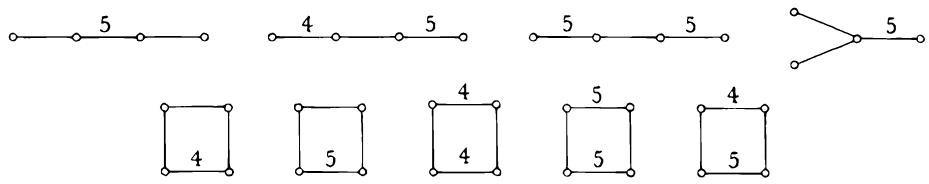
\includegraphics[keepaspectratio]{images/part001_8fab2eba.jpg}}

\begin{enumerate}
\def\labelenumi{\alph{enumi})}
\setcounter{enumi}{1}
\tightlist
\item
  对秩 5 回答同样的问题，其清单由下列五个图组成：
\end{enumerate}

\pandocbounded{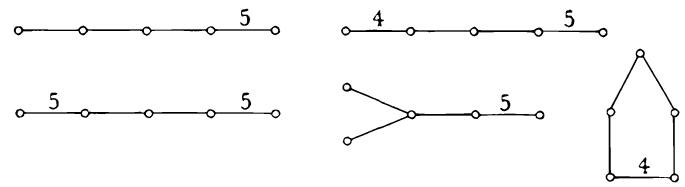
\includegraphics[keepaspectratio]{images/part001_6b3cac07.jpg}}

\begin{enumerate}
\def\labelenumi{\alph{enumi})}
\setcounter{enumi}{2}
\tightlist
\item
  证明不存在秩 \(\geqslant 6\) 的紧双曲型图。*
\end{enumerate}

\begin{enumerate}
\def\labelenumi{\arabic{enumi})}
\setcounter{enumi}{15}
\tightlist
\item
  *证明：任何有一条系数为 6 的棱的、秩 \(\geqslant 4\) 的双曲型 Coxeter 图都同构于下列十一个图之一（它们是非紧的且秩为 4）：
\end{enumerate}

\pandocbounded{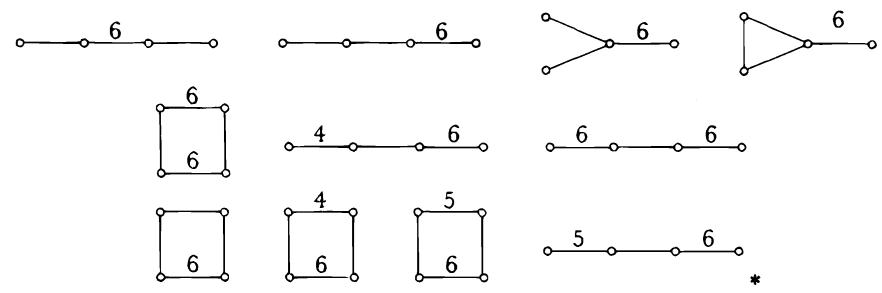
\includegraphics[keepaspectratio]{images/part001_2926a96c.jpg}}

\begin{enumerate}
\def\labelenumi{\arabic{enumi})}
\setcounter{enumi}{16}
\tightlist
\item
  *证明：更高秩的双曲 Coxeter 图是下列三个图（它们的秩为 10）：
\end{enumerate}

\pandocbounded{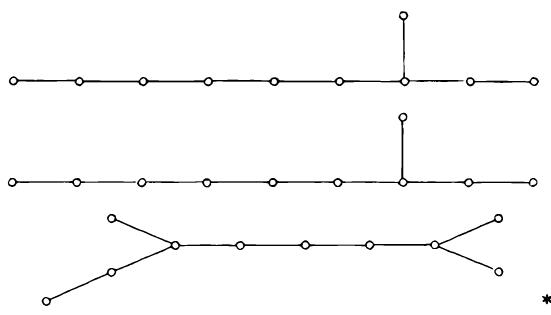
\includegraphics[keepaspectratio]{images/part001_3a8f46b0.jpg}}

¶ 18) 假设 (W,S) 是双曲型的，且 W 使 E 的一个格 \(\Gamma\) 稳定。设 G 是 \(B_{M}\) 的正交群，设 \(G(\Gamma)\) 是元素 \(g \in G\)（满足 \(g\Gamma = \Gamma\)）组成的子群。证明 \(G(\Gamma)\) 是 G 的离散子群。证明 W 是 \(G(\Gamma)\) 的有限指数子群（利用 W\textbackslash G 的测度有限这一事实）。

*若 (W, S) 实际上是紧双曲型的，证明相应的 Coxeter 图同构于下列图之一（使用 Exercs. 4, 6 与 15）：

\pandocbounded{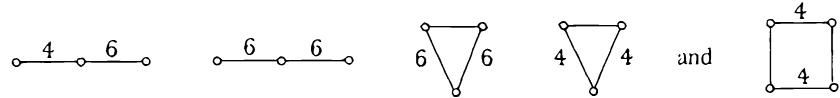
\includegraphics[keepaspectratio]{images/part001_0d92fd3d.jpg}}

证明与 Exerc. 16 的图（最后四个除外）相应的群都使一个格稳定（使用 Exerc. 6 的方法）。*

\begin{enumerate}
\def\labelenumi{\arabic{enumi})}
\setcounter{enumi}{18}
\tightlist
\item
  设 \((W,S)\) 是与图
\end{enumerate}

\pandocbounded{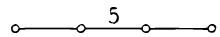
\includegraphics[keepaspectratio]{images/part001_8b3dcc37.jpg}}

相应的 Coxeter 系统。它是一个紧双曲型的系统（cf.~Exerc. 15）。型 \(B_{M}\) 关于基 \((e_{s})\) 的系数属于域 \(\mathbf{Q}(\sqrt{5})\) 中由该域的在 Z 上整的元素组成的子环 A。

\begin{enumerate}
\def\labelenumi{\alph{enumi})}
\item
  设 \(\sigma\) 是 \(K\) 到 \(\mathbf{R}\) 中的、把 \(\sqrt{5}\) 映为 \(-\sqrt{5}\) 的嵌入。证明 \(\sigma(B_M)\)（型 \(B_M\) 在 \(\sigma\) 下的像）非退化且正。
\item
  设 G 是 \(B_{M}\) 的正交群，\(G_{\sigma}\) 是 \(\sigma(B_{M})\) 的正交群。设 \(G_{A}\) 是 G 中由关于 \((e_{s})\) 的矩阵系数在 A 中的元素组成的子群。证明 \(G_{A}\) 可与 \(G \times G_{\sigma}\) 的一个离散子群等同，然后利用 a) 证明 \(G_{A}\) 是 G 的离散子群。
\item
  证明 W 是 \(G_{A}\) 的一个有限指数子群。
\end{enumerate}

\(d)\) 对 Exerc. 15 中的其余图证明类似的结果（域 \(\mathbf{Q}(\sqrt{5})\) 有时换成 \(\mathbf{Q}(\sqrt{2})\)），但下面的图除外：

\pandocbounded{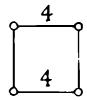
\includegraphics[keepaspectratio]{images/part001_99b486d1.jpg}}

即 Exerc. 18 中处理的图，以及图 \(^{8}\)

\pandocbounded{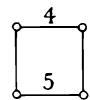
\includegraphics[keepaspectratio]{images/part001_2a5e784a.jpg}}

¶ 20) 对 S 的每个子集 \(\{s, s'\}\)（满足 \(m(s, s') = \infty\)），设 \(r(s, s')\) 是一个实数 \(\leqslant -1\)。给 E 赋以双线性型 \(\mathbf{B}_r\)，使得

\[
\begin{array}{l l} \mathrm{B} _ {r} (e _ {s}, e _ {s ^ {\prime}}) = \mathrm{B} _ {\mathrm{M}} (e _ {s}, e _ {s ^ {\prime}}) = - \cos \frac {\pi}{m (s , s ^ {\prime})} & \text {if} m (s, s ^ {\prime}) \neq \infty \\ \mathrm{B} _ {r} (e _ {s}, e _ {s ^ {\prime}}) = r (s, s ^ {\prime}) & \text {if} m (s, s ^ {\prime}) = \infty . \end{array}
\]

与 \(B_{M}\) 的情形一样，我们定义反射 \(\sigma_{s}\)，它以 \(e_{s}\) 为向量，且使型 \(B_{r}\) 不变。

\begin{enumerate}
\def\labelenumi{\alph{enumi})}
\item
  证明存在唯一的同态 \(\sigma_r: \mathbf{W} \to \mathbf{GL}(\mathbf{E})\)，使得 \(\sigma_r(g_s)\) 等于上面定义的反射 \(\sigma_s\)。
\item
  证明 Prop. 4、Th. 1 及其诸系、以及 Lemma 1 中的断言对 \(\sigma_r\) 仍然成立。
\end{enumerate}

\exercisesection{§ 5 的习题}

\begin{enumerate}
\def\labelenumi{\arabic{enumi})}
\item
  确定一个有限二面体群的对称不变元代数（就其 2 维典范表示而言，cf.~§4, no. 2）。
\item
  设 A 是一个主理想环，E 是一个有限秩 l 的自由 A-模，G 是 \(\mathbf{GL}(\mathbf{E})\) 的一个有限子群。假设：
\end{enumerate}

\begin{enumerate}
\def\labelenumi{(\roman{enumi})}
\item
  若 \(q = \operatorname{Card}(G)\)，则元素 \(q.1\)（\(A\) 中的元素）可逆。
\item
  G 由 E 中的伪反射生成（即由使 \((s - 1)(E)\) 是 E 的一个单生成子模的元素 s 生成，cf.~§2, Exerc. 1。）
\end{enumerate}

设 \(\mathbf{S}(\mathrm{E})\) 是 \(\mathrm{E}\) 的对称代数，\(\mathbf{S}(\mathrm{E})^{\mathrm{G}}\) 是 \(\mathbf{S}(\mathrm{E})\) 中由在 \(\mathrm{G}\) 下不变的元素组成的子代数。证明：对从 \(\mathrm{A}\) 到域 \(k\) 中的任何同态，\(\mathbf{S}(\mathrm{E})^{\mathrm{G}} \otimes k\) 可与 \(\mathbf{S}(\mathrm{E} \otimes k)^{\mathrm{G}}\) 等同。由此，应用 Th. 4 推出，\(\mathbf{S}(\mathrm{E})^{\mathrm{G}}\) 是 \(\mathrm{A}\) 上的一个分次多项式代数。

¶ 3) 设 K 是一个特征为零的域，V 是 K 上一个有限维 l 的向量空间，G 是 GL(V) 的一个由伪反射生成的子群。置 q = Card(G)；用 S（相应地，L）表示 V 的对称代数（相应地，外代数）。若 \(x \in V\)，用 x（相应地，\(x'\)）表示它在 S（相应地，L）中的典范像。

\begin{enumerate}
\def\labelenumi{\alph{enumi})}
\item
  设 \(E = S \otimes L\) 是 S 与 L 的张量积。证明 E 上存在唯一的导子 d，使得 \(dx = x'\) 且 \(dx' = 0\) 对所有 \(x \in V\) 成立。
\item
  设 \(S^{G}\) 是 G 的对称不变元代数，\(P_{1},\ldots,P_{l}\) 是 \(S^{G}\) 中使 \(S^{G}=K[P_{1},\ldots,P_{l}]\) 的齐次元素。对每个子集 \(I=\{i_{1},\ldots,i_{r}\}\)（\([1,l]\) 的、满足 \(i_{1}<\cdots<i_{r}\) 的子集），置
\end{enumerate}

\[
\omega_ {\mathrm{I}} = d \mathrm{P} _ {i _ {1}} \dots d \mathrm{P} _ {i _ {r}}.
\]

证明诸 \(\omega_{I}\) 在 S 上线性无关，且都属于 E 中由在 G 下不变的元素组成的子代数 \(E^{G}\)。由此推出，对所有 \(\omega \in E^{G}\)，存在 \(a, c_{I} \in S^{G}\)，其中 \(a \neq 0\)，使得

\[
a \omega = \sum_ {\mathrm{I}} c _ {\mathrm{I}} \omega_ {\mathrm{I}}.
\]

\(c)\) 证明 \(\mathrm{E}^{\mathrm{G}}\) 中包含在 \(S\otimes \bigwedge^{l}\mathrm{V}\) 中的每个元素都形如 \(c.dP_{1}\ldots dP_{l}\)，其中 \(c\in S^{\mathrm{G}}\)。（应用 Prop. 5。）

\begin{enumerate}
\def\labelenumi{\alph{enumi})}
\setcounter{enumi}{3}
\item
  证明诸 \(\omega_{I}\) 构成 \(S^{G}\)-模 \(E^{G}\) 的基。（用 b) 的记号，把关系式 \(a\omega = \sum_{I} c_{I}\omega_{I}\) 的两边乘以一个元素 \(\omega_{J}\)，并应用 c)；由此推出，若 I 是 J 的余集，则 a 整除 \(c_{I}\)；从而 \(^{9}\) 诸 \(\omega_{I}\) 生成 \(E^{G}\)。）
\item
  设 \(S_{n}\)（相应地，\(L_{m}\)）是 \(S\)（相应地，\(L\)）的 \(n\) 次（相应地，\(m\) 次）齐次分量。置
\end{enumerate}

\[
\begin{array}{r l r} & & {\mathrm{E} _ {n, m} = \mathrm{S} _ {n} \otimes \mathrm{L} _ {m}, \quad \mathrm{E} _ {n, m} ^ {\mathrm{G}} = \mathrm{E} ^ {\mathrm{G}} \cap \mathrm{E} _ {n, m}, \quad a _ {n, m} = \dim \mathrm{E} _ {n, m} ^ {\mathrm{G}},} \\ & & {a (\mathrm{X}, \mathrm{Y}) = \sum_ {n, m \geqslant 0} a _ {n, m} \mathrm{X} ^ {n} \mathrm{Y} ^ {m}.} \end{array}
\]

利用 \(d\) )，证明公式

\[
a (\mathrm{X}, \mathrm{Y}) = \prod_ {i = 1} ^ {l} \frac {1 + \mathrm{Y} . \mathrm{X} ^ {p _ {i} - 1}}{1 - \mathrm{X} ^ {p _ {i}}},
\]

其中 \(p_{i} = \deg(P_{i})\)。

\(f)\) 若 \(g \in \mathbf{G}\)，用 \(\operatorname{Tr}_{n,m}(g)\) 表示 \(\mathbf{E}_{n,m}\) 的、由 \(g\) 所定义的自同构的迹；置

\[
\operatorname{Tr} (\mathrm{X}, \mathrm{Y}) (g) = \sum_ {n, m \geqslant 0} \operatorname{Tr} _ {n, m} (g) \mathrm{X} ^ {n} \mathrm{Y} ^ {m}.
\]

证明

\[
\operatorname{Tr} (X, Y) (g) = \frac {\det (1 + Y g)}{\det (1 - X g)}.
\]

\begin{enumerate}
\def\labelenumi{\alph{enumi})}
\setcounter{enumi}{6}
\tightlist
\item
  设 \(q = \operatorname{Card}(\mathbf{G})\)。证明
\end{enumerate}

\[
\frac {1}{q} \sum_ {g \in G} \operatorname{Tr} (X, Y) (g) = a (X, Y),
\]

即

\[
\frac {1}{q} \sum_ {g \in G} \frac {\det (1 + Y g)}{\det (1 - X g)} = \prod_ {i = 1} ^ {l} \frac {1 + Y . X ^ {p _ {i} - 1}}{1 - X ^ {p _ {i}}}.
\]

（利用下列结果：若 \(\mathbf{G}\) 作用在一个有限维向量空间 \(\mathbf{E}\) 上，则 \(\mathbf{E}\) 中在 \(\mathbf{G}\) 下不变的元素所成空间的维数等于 \(\frac{1}{q}\sum_{g\in \mathbf{G}}\mathrm{Tr}_{\mathbf{E}}(g).\)）

当 Y = 0 时这个公式给出什么？

\begin{enumerate}
\def\labelenumi{\alph{enumi})}
\setcounter{enumi}{7}
\tightlist
\item
  对任何整数 \(p \geqslant 0\)，设 \(H_{p}\) 是 G 中以 1 为重数 p 的特征值的元素 \(g \in G\) 组成的集合。~设 \(h_{p} = \text{Card}(H_{p})\)。证明公式
\end{enumerate}

\[
\sum_ {p = 0} ^ {l} h _ {p} \mathbf {T} ^ {p} = \prod_ {i = 1} ^ {l} (p _ {i} - 1 + \mathbf {T}).
\]

（在上面的 \(g\) ) 中的公式里，把 \(Y\) 换成 \(-1 + T(1 - X)\)，然后在所得结果中置 \(X = 1\)。若 \(g \in H_p\)，则项 \(\operatorname{Tr}(X, Y)(g)\) 变成 \(T^p\)。）

¶ 4) *设 \(G _ {1} = \mathbf {S L} _ {3} (\mathbf {F} _ {2})\)。

\begin{enumerate}
\def\labelenumi{\alph{enumi})}
\item
  证明 \(\mathbf{G}_1\) 是一个 168 阶的非交换单群，含有 21 个 2 阶元素。
\item
  证明 \(G_{1}\) 的不可约复表示的次数是 1, 3, 3, 6, 7, 8。
\item
  设 \(\rho: \mathbf{G}_1 \to \mathbf{GL}_3(\mathbf{C})\) 是一个不可约表示 \(^{10}\)，它是 \(\mathbf{G}_1\) 的 3 次表示。若 \(y \in \mathbf{G}_1\) 是 2 阶的，证明 \(\operatorname{Tr}(\rho(y)) = -1\)。由此推出 \(-\rho(y)\) 是一个反射。
\item
  设 G 是 \(\mathbf{GL}_{3}(\mathbf{C})\) 中由诸元素 \(-\rho(y)\)（y 取遍 \(G_{1}\) 中的 2 阶元）生成的子群。证明 G 同构于 \(G_{1} \times \{1, -1\}\)，从而其阶为 336。
\item
  证明特征次数 \(k_{1}, k_{2}, k_{3}\)（\(\mathbf{G}\) 的对称不变元代数的特征次数）等于 4、6 与 14。（利用关系式 \(\prod_{i} k_{i} = 336\) 与 \(\sum_{i} (k_{i} - 1) = 21\)。）
\item
  证明 G 不是一个 Coxeter 群。*
\end{enumerate}

\begin{enumerate}
\def\labelenumi{\arabic{enumi})}
\setcounter{enumi}{4}
\tightlist
\item
  *设 \(K\) 是一个域，\(S = K[X_1, \ldots, X_n]\) 是 \(K\) 上的一个分次多项式代数，由代数无关的齐次元素 \(X_i\)（次数 \(> 0\)）生成。
\end{enumerate}

\begin{enumerate}
\def\labelenumi{\alph{enumi})}
\tightlist
\item
  设 \(Y_{1},\ldots,Y_{n}\) 是 S 中次数 \textgreater0 的齐次元素，\(R = K[Y_{1},\ldots,Y_{n}]\) 是 S 中由这些元素生成的子代数。证明下列性质等价：
\end{enumerate}

\begin{enumerate}
\def\labelenumi{(\roman{enumi})}
\item
  \((\mathrm{Y}_1,\dots ,\mathrm{Y}_n)\) 是一个 S-正则序列。
\item
  S 在 R 上是整的。
\item
  \(S\) 中由 \(Y_{1},\ldots ,Y_{n}\) 生成的理想在 \(S\) 中有有限余维数。
\item
  对任何扩张 \(\overline{\mathbf{K}}\)（\(\mathbf{K}\) 的扩张），方程组 \(Y_{i}(x_{1},\ldots ,x_{n}) = 0\)（\(1\leqslant i\leqslant n\)，\(x_{i}\in \overline{\mathbf{K}}\)）只有平凡解 \((0,\dots ,0)\)。
\end{enumerate}

\(((\mathrm{i}) \Longleftrightarrow (\mathrm{iii})\) 由 Macaulay 的一个定理得出（Commutative Algebra）；\((\mathrm{iii}) \Longleftrightarrow (\mathrm{iv})\) 由零点定理得出（Commutative Algebra, Chap. V, §3, no. 3, Prop. 2）；(ii) \(\Longleftrightarrow (\mathrm{iii})\) 是容易的。）

若这些性质满足，证明诸 \(Y_{i}\) 在 K 上代数无关，且 S 是一个自由 R-模，其秩等于

\[
\frac {\prod_ {i} \deg (\mathrm{Y} _ {i})}{\prod_ {i} \deg (\mathrm{X} _ {i})}.
\]

\begin{enumerate}
\def\labelenumi{\alph{enumi})}
\setcounter{enumi}{1}
\tightlist
\item
  设 G 是分次代数 S 的一个有限自同构群，\(S^{G}\) 是它的不变元子代数，\(Y_{1},\ldots,Y_{n}\) 是 \(S^{G}\) 中满足上面条件 (i),\ldots, (iv) 的元素。证明 \(S^{G}=K[Y_{1},\ldots,Y_{n}]\) 当且仅当
\end{enumerate}

\[
\operatorname{Card} (\mathrm{G}) = \frac {\prod_ {i} \deg \left(\mathrm{Y} _ {i}\right)}{\prod_ {i} \deg \left(\mathrm{X} _ {i}\right)}. *
\]

¶ 6) *设 n 是一个整数 ≥ 1，q 是一个素数的幂，K = F\_q，V = K\^{}n，G = GL(n, K)，G\_1 = SL(n, K)。把 G 与群 GL(V) 等同。此外，用 S 表示代数 S(V) = K{[}X\_1, \ldots, X\_n{]}，用 R（相应地，R\_1）表示 S 中由在 G（相应地，G\_1）下不变的元素组成的子代数。

\begin{enumerate}
\def\labelenumi{\alph{enumi})}
\tightlist
\item
  设 \(\mathbf{e} = (e_1, \ldots, e_n)\) 是一个整数序列 \(\geqslant 0\)。置
\end{enumerate}

\[
\mathrm{L} _ {\mathbf {e}} = \det (\mathrm{X} _ {i} ^ {q ^ {e _ {j}}}).
\]

这是 \(S\) 的一个元素。

证明

\[
g. \mathrm{L} _ {\mathbf {e}} = \det (g) \mathrm{L} _ {\mathbf {e}} \text {for all} g \in \mathrm{G}.
\]

（注意，若 \(g.X_i = \sum_j a_{ij} X_j\)，则 \(g.X_i^{q^e} = \sum_j a_{ij} X_j^{q^e}\)。）特别地，\(L_e\) 属于 \(R_1\)。

\begin{enumerate}
\def\labelenumi{\alph{enumi})}
\setcounter{enumi}{1}
\tightlist
\item
  设 \(j \in [1, n]\)。置
\end{enumerate}

\[
Z _ {j} = \prod_ {(a _ {i j})} (X _ {j} + \sum_ {i > j} a _ {i j} X _ {i}),
\]

其中乘积取遍 K 的元素的所有族 \((a_{ij})_{j < i\leqslant n}\)。设

\[
\mathrm{T} = \prod_ {j = 1} ^ {n} Z _ {j}.
\]

证明 T 整除所有 \(L_{e}\)。由此推出 \(T = L_{e_{n}}\)，其中 \(e_{n} = (0, 1, \ldots, n - 1)\)，且 T 在 \(G_{1}\) 下不变。

\begin{enumerate}
\def\labelenumi{\alph{enumi})}
\setcounter{enumi}{2}
\tightlist
\item
  用 \(\mathbf{e}_i\)（\(1 \leqslant i \leqslant n - 1\)）表示序列 \((0, 1, \ldots, i - 1, i + 1, \ldots, n)\)，并置 \(\mathrm{Y}_i = \mathrm{L}_{\mathbf{e}_i} / \mathrm{T}\)，cf.~b)。证明诸 \(\mathrm{Y}_i\) 属于 R 且 \(\deg(\mathrm{Y}_i) = q^n - q^i\)。
\end{enumerate}

\(d)\) 设 \(S' = K[X_1, \ldots, X_{n-1}]\)，并设 \(T', Y_1', \ldots, Y_{n-2}'\) 是 \(S'\) 中以与 \(T, Y_1, \ldots, Y_{n-1}\) 同样的方式（但把 \(n\) 换成 \(n-1\)）定义的元素。设 \(f: S \to S'\) 是由

\[
f \left(\mathrm{X} _ {i}\right) = \mathrm{X} _ {i} (1 \leqslant i \leqslant n - 1), f \left(\mathrm{X} _ {n}\right) = 0.
\]

定义的同态。证明

\[
f (\mathrm{T}) = 0, \quad f (\mathrm{Y} _ {1}) = \mathrm{T} ^ {\prime q (q - 1)}, \quad f (\mathrm{Y} _ {i}) = \mathrm{Y} _ {i - 1} ^ {\prime q} \quad \text{对} \quad 2 \leqslant i \leqslant n - 1.
\]

\begin{enumerate}
\def\labelenumi{\alph{enumi})}
\setcounter{enumi}{4}
\tightlist
\item
  证明族 \((T, Y_{1}, \ldots, Y_{n-1})\) 满足 Exerc. 5 的条件 (iv)。（设 \(x = (x_{1}, \ldots, x_{n})\) 是方程组 \((T, Y_{1}, \ldots, Y_{n-1})\) 在 K 的一个扩张 \(\overline{K}\) 中的一个零点。由于 x 是 T 的零点，诸 \(x_{i}\) 满足至少一个系数在 K 中的非平凡线性关系。必要时用 \(G_{1}\) 的一个元素变换 x，可以假设 \(x_{n} = 0\)。应用 d) 并对 n 用归纳法完成证明。）
\end{enumerate}

\(f)\) 证明 \(\mathbf{R}_1 = \mathbf{K}[\mathbf{T},\mathbf{Y}_1,\dots ,\mathbf{Y}_{n - 1}]\)，且 \(\mathrm{T},\mathrm{Y}_1,\dots ,\mathrm{Y}_{n - 1}\) 代数无关（“Dickson 定理”——应用 e) 与 Exerc. 5，并注意 \(\mathbf{G}_1\) 的阶等于 \(\deg (\mathrm{T}) = \sum_{i}\deg (\mathrm{Y}_i)\)）。

\begin{enumerate}
\def\labelenumi{\alph{enumi})}
\setcounter{enumi}{6}
\tightlist
\item
  证明 \(R = K[T^{q-1}, Y_{1}, \ldots, Y_{n-1}]\)。
\end{enumerate}

¶ 7) *设 R 是一个正则局部环（Commutative Algebra, Chap. VIII, §5, no. 1），其极大理想为 m，剩余域为 k。设 G 是 R 的一个有限自同构群，\(R' = R^{G}\) 是 R 中由在 G 下不变的元素组成的子环。这是一个局部环，其极大理想为 \(m' = m \cap R'\)。假设：

\begin{enumerate}
\def\labelenumi{(\roman{enumi})}
\item
  \(R'\) 是诺特的，且 R 是一个有限型 \(R'\)-模。
\item
  复合映射 \(R'\to R\to k\) 是满射。
\end{enumerate}

置 \(V = \mathfrak{m} / \mathfrak{m}^2\)；这是一个 \(k\)-向量空间。\(G\) 在 \(R\) 上的作用定义了一个同态 \(\varepsilon : G \to \mathbf{GL}(V)\)。

\begin{enumerate}
\def\labelenumi{\alph{enumi})}
\item
  设 \(\mathfrak{p}\) 是 \(R\) 的一个高度为 1 的素理想（Commutative Algebra, Chap. VII, §1, no. 6），\(s \in G\) 满足 \(s(\mathfrak{p}) = \mathfrak{p}\) 且 \(s\) 平凡地作用在 \(R / \mathfrak{p}\) 上。证明 \(\varepsilon(s)\) 是 \(V\) 的一个伪反射。（注意 \(\mathfrak{p}\) 在 \(\mathfrak{m} / \mathfrak{m}^2\) 中的像的维数是 0 或 1。）
\item
  证明：若 \(R'\) 正则，则子群 \(\varepsilon(G)\)（\(\mathbf{GL}(V)\) 的子群）由伪反射生成。（设 H 是 G 中由其在 \(\varepsilon\) 下的像为伪反射的元素生成的子群，\(R^{H}\) 是 R 中由在 H 下不变的元素组成的子环。利用 a) 证明：\(R'\) 的任何高度为 1 的素理想都不在 \(R^{H}\) 中分歧；利用 \(R^{H}\) 是整闭的这一事实，借助纯性定理 \(^{11}\) 推出 \(R' = R^{H}\)，从而 H = G。）
\item
  现在设 \(\mathbf{G}\) 的阶与 \(k\) 的特征互素。证明 \(\varepsilon\) 是单射。
\end{enumerate}

设 \((\mathfrak{m}_{n}^{\prime})\) 是 \(R^{\prime}\) 的、由 R 的 m-进滤链 \((\mathfrak{m}^{n})\) 诱导的滤链，并设

\[
i: \mathrm{gr} (\mathrm{R} ^ {\prime}) \to \mathrm{gr} (\mathrm{R})
\]

是从 \(R'\) 的相伴分次代数到 R 的相伴分次代数的典范同态（Commutative Algebra, Chap. III, §2）。证明 i 是单射，且它的像是子环 \(\mathrm{gr}(R)^{\mathrm{G}}\)，即 \(\mathrm{gr}(R)\) 中由在 G 下不变的元素组成的子环。

\(d)\) 沿用 \(c\) ) 的假设与记号，并进一步假设 \(\varepsilon (\mathbf{G})\) 由伪反射生成。若 \(l = \dim V\)，设 \(\mathrm{P}_1,\ldots ,\mathrm{P}_l\) 是 \(k\)-代数 \(\mathrm{gr}(R)^{\mathrm{G}}\) 的代数无关的齐次生成元（由 Th. 4 以及 \(\mathrm{gr}(R)\) 可与 V 的对称代数等同这一事实，这样的元素存在）；设 \(p_1,\ldots ,p_l\) 是它们的次数。由 \(c\) )，可以找到 \(x_{i}\in \mathfrak{m}_{p_{i}}^{\prime}\) 使得 \(\mathrm{gr}(x_i) = \mathrm{P}_i\)。证明诸 \(x_{i}\) 生成理想 \(\mathfrak{m}'\)，并由此推出 \(R'\) 是正则的。*

¶ 8) *设 V 是域 K 上一个有限维向量空间，S 是 V 的对称代数，G 是 GL(V) 的一个有限子群。假设代数 \(S^G\)（\(G\) 的对称不变量组成的代数）是一个分次多项式代数。

\begin{enumerate}
\def\labelenumi{\alph{enumi})}
\tightlist
\item
  设 u 是 V 的对偶 \(V^{*}\) 的一个元素，\(G_{u}\) 是 G 中由使 u 不变的元素组成的子群。证明 \(G_{u}\) 由伪反射生成。（线性型 u 可扩张为一个同态 \(f_{u}: S \to K\)。若用 \(S_{u}\) 表示 S 关于 \(f_{u}\) 的核的局部环，则环 \(S_{u}\) 是正则的。把 Exerc. 7 b) 应用于 \(G_{u}\)（把它视为 \(S_{u}\) 的自同构群），即得结论。）
\end{enumerate}

特别地，G 由伪反射生成。

\begin{enumerate}
\def\labelenumi{\alph{enumi})}
\setcounter{enumi}{1}
\tightlist
\item
  设 A 是 \(V^{*}\) 的一个子集，\(G_{A} = \bigcap_{u \in A} G_{u}\)。证明 \(G_{A}\) 由伪反射生成。（必要时扩张基域，可以假设 K 无限。证明在此情形下，存在由 A 生成的 \(V^{*}\) 的向量子空间中的一个元素 v，使得 \(G_{v} = G_{A}\)。对 \(v\) 应用 a) 即得结论。）
\end{enumerate}

\begin{enumerate}
\def\labelenumi{\arabic{enumi})}
\setcounter{enumi}{8}
\tightlist
\item
  设 V 是有限域 K（特征异于 2）上一个 4 维向量空间，Q 是 V 上一个指数为 2 的非退化二次型（Algebra, Chap. IX, §4, no. 2）。设 G = O(Q) 是这个型的正交群；这是一个由反射生成的有限群（loc. cit., §6, no. 4, Prop. 5）。
\end{enumerate}

\begin{enumerate}
\def\labelenumi{\alph{enumi})}
\item
  设 E 是 V 的一个极大全迷向子空间，\(G_{E}\) 是 G 中由使 \(g(x) = x\)（对所有 \(x \in E\)）的元素 g 组成的子群。证明 \(G_{E}\) 同构于 K 的加法群，且不含任何伪反射。
\item
  证明 G 的对称不变元代数不是一个分次多项式代数（利用前一习题）。
\end{enumerate}

\exercisesection{§ 6 的习题}

在下面的习题中（Exerc. 3 除外），假设与记号均取自 §6。

\begin{enumerate}
\def\labelenumi{\arabic{enumi})}
\item
  假设 W 不可约。设 c 是 W 的一个 Coxeter 变换，\(\Gamma\) 是 W 中由 c 生成的子群，\(\Delta\) 是与 H 的某个元素正交的单位向量组成的集合。证明 \(\Gamma\) 在 \(\Delta\) 中有 l 个轨道，且每个轨道有 h 个元素。（按 Chap. VI, §1, no. 11 的 Prop. 33 的证明方式论证。）
\item
  假设 W 不可约。设 C 是相对于 W 的一个室，\((\mathrm{H}_{1},\ldots,\mathrm{H}_{l})\) 是它的墙，\(e_{i}\) 是与 \(H_{i}\) 正交的一个非零向量。假设 \(e_{1},\ldots,e_{r}\)（相应地，\(e_{r+1},\ldots,e_{l}\)）两两正交（cf.~no. 2）。对所有 \(u\in Z\)，定义 \(H_{u}\) 与 \(s_{u}\) 如下：\(H_{u}=H_{k}\)（若 \(u\equiv k\pmod{l}\)），且 \(s_{u}=s_{H_{u}}\)。
\end{enumerate}

\begin{enumerate}
\def\labelenumi{\alph{enumi})}
\item
  证明 \(\mathfrak{H}\) 的元素正是诸 \(s_1 s_2 \ldots s_{u-1} H_u\)，其中 \(u = 1, 2, \ldots, lh/2\)。
\item
  设 \(s' = s_1 \ldots s_r\)，\(s'' = s_{r+1} \ldots s_l\)，于是 \(c = s's''\) 是与有序室 C 相伴的 Coxeter 变换。设 \(w_0\) 是 W 中把 C 变到 -C 的元素（cf.~§4, Exerc. 2）。证明：若 \(h\) 为奇数，则
\end{enumerate}

\[
w _ {0} = \underbrace {s ^ {\prime} s ^ {\prime \prime} s ^ {\prime} \ldots s ^ {\prime \prime} s ^ {\prime}} _ {h \text {terms}} = \underbrace {s ^ {\prime \prime} s ^ {\prime} s ^ {\prime \prime} \ldots s ^ {\prime} s ^ {\prime \prime}} _ {h \text {terms}} = s ^ {\prime \prime} c ^ {(h - 1) / 2} = c ^ {(h - 1) / 2} s ^ {\prime}.
\]

\begin{enumerate}
\def\labelenumi{\alph{enumi})}
\setcounter{enumi}{2}
\tightlist
\item
  置 \(S = \{s_1, \ldots, s_l\}\)。偶 (W,S) 是一个 Coxeter 系统。若 \(w \in W\)，用 \(l_S(w)\) 表示 \(w\) 关于 S 的长度（Chap. IV, §1, no. 1）。证明
\end{enumerate}

\[
l _ {\mathrm{S}} (s ^ {\prime}) = r, l _ {\mathrm{S}} (s ^ {\prime \prime}) = l - r, l _ {\mathrm{S}} (c) = l.
\]

在 b) 的假设下，由此推出

\[
l _ {\mathrm{S}} (w _ {0}) \leqslant r + \frac {h - 1}{2} l \text { and } l _ {\mathrm{S}} (w _ {0}) \leqslant (l - r) + \frac {h - 1}{2} l.
\]

另一方面，证明 \(l_{S}(w_0) = \mathrm{Card}(\mathfrak{H}) = hl / 2\)（使用 Chap. IV, §1 的 Exerc. 22）。由此推出 \(r = l / 2\)，且 \((s_1, s_2, \ldots, s_{lh / 2})\) 是 \(w_0\) 的一个约化分解。

\(d)\) 证明：若 \(h\) 为偶数，则 \((s_1,\ldots ,s_{lh / 2})\) 是 \(w_{0} = c^{h / 2}\) 的一个约化分解。（方法同上。）

¶ 3) 设 K 是一个交换环，E 是一个以 \((e_1, \ldots, e_l)\) 为基的自由 K-模，\(f_1, \ldots, f_l\) 是 E 的对偶中的元素。置 \(a_{ij} = f_i(e_j)\)。若 \(1 \leqslant i \leqslant l\)，设 \(s_i\) 是伪反射 \(s_{e_i, f_i}\)（\S 2, Exerc. 1）。则

\[
s _ {i} (e _ {j}) = e _ {j} - a _ {i j} e _ {i}.
\]

置 \(c = s_1 \ldots s_l\)，\(z_i = c(e_i)\)。

\begin{enumerate}
\def\labelenumi{\alph{enumi})}
\tightlist
\item
  对 \(1 \leqslant i, k \leqslant l\)，置
\end{enumerate}

\[
y _ {i} ^ {k} = s _ {1} \dots s _ {k} (e _ {i}) \text { and } y _ {i} = s _ {1} \dots s _ {i - 1} (e _ {i}) = y _ {i} ^ {i - 1}.
\]

于是 \(y_{i}^{0} = e_{i}\)，\(y_{i}^{l} = z_{i}\)。

证明

\[
y _ {i} ^ {k - 1} - y _ {i} ^ {k} = a _ {k i} y _ {k}.
\]

由此推出公式

\[
e _ {i} = y _ {i} + \sum_ {k <   i} a _ {k i} y _ {k}
\]

\[
z _ {i} = y _ {i} - \sum_ {k \geqslant i} a _ {k i} y _ {k}.
\]

\begin{enumerate}
\def\labelenumi{\alph{enumi})}
\setcounter{enumi}{1}
\tightlist
\item
  设 C 是 \(c\) 关于基 \((e_i)\) 的矩阵。设 \(U = (u_{ij})\) 与 \(V = (v_{ij})\) 是由下式定义的矩阵
\end{enumerate}

\[
u _ {i j} = \left\{ \begin{array}{l l} a _ {i j} & \text { if } i <   j \\ 0 & \text { otherwise, } \end{array} \right. v _ {i j} = \left\{ \begin{array}{l l} 0 & \text { if } i <   j \\ a _ {i j} & \text { otherwise. } \end{array} \right.
\]

矩阵 \(\mathrm{I} + \mathrm{U}\) 可逆且行列式为 1。证明

\[
\mathrm{C} = (\mathrm{I} - \mathrm{V}) (\mathrm{I} + \mathrm{U}) ^ {- 1}.
\]

由此推出

\[
\det (\lambda I - C) = \det ((\lambda - 1) I + V + \lambda U),
\]

换句话说

\[
\det (\lambda \mathrm{I} - \mathrm{C}) = \left| \begin{array}{c c c c c} (\lambda - 1) + a _ {1 1} & \lambda a _ {1 2} & \lambda a _ {1 3} & \dots & \lambda a _ {1 l} \\ a _ {2 1} & \lambda (\lambda - 1) + a _ {2 2} & \lambda a _ {2 3} & \dots & \lambda a _ {2 l} \\ a _ {3 1} & a _ {3 2} & (\lambda - 1) + a _ {3 3} & \dots & \lambda a _ {3 l} \\ \vdots & \vdots & \vdots & \ddots & \vdots \\ a _ {l 1} & a _ {l 2} & a _ {l 3} & \dots & (\lambda - 1) + a _ {l l} \end{array} \right|.
\]

\begin{enumerate}
\def\labelenumi{\alph{enumi})}
\setcounter{enumi}{2}
\tightlist
\item
  设 \(\Gamma = (\mathrm{I},\mathrm{S})\) 是这样的图：其顶点集为 \(\mathrm{I} = [1,l]\)，其棱集 S 是 I 的二元子集 \(\{i,j\}\)（满足 \(a_{ij}\neq 0\) 或 \(a_{ji}\neq 0\)）组成的集合。若 \(\alpha = \{i,j\}\) 属于 S，用 \(\sigma_{\alpha}\) 表示 \(i\) 与 \(j\) 的对换（视为对称群 \(\mathrm{S_I}\) 的元素），并置 \(a_{\alpha} = -a_{ij}a_{ji}\)。
\end{enumerate}

设 \(\mathfrak{B}\) 是 \(S\) 中由顶点两两不交的棱组成的子集的集合。若 \(X \in \mathfrak{B}\)，用 \(C(X)\) 表示所有这样的 \(i \in I\)（它们不是 \(X\) 的任何棱的顶点）组成的集合，并置 \(\sigma_X = \prod_{\alpha \in X} \sigma_\alpha\)，\(a_X = \prod_{\alpha \in X} a_\alpha\)。

设 \(\sigma \in S_{I}\)，\(d_{\sigma}\) 是与 \(\sigma\) 对应的项（在 \((\lambda - 1)I + V + \lambda U\) 的行列式展开式中）。证明：若 \(\sigma\) 形如 \(\sigma_{X}\)，其中 \(X \in \mathfrak{B}\)，则

\[
d _ {\sigma} = a _ {X} \lambda^ {\operatorname{Card} (X)} \prod_ {i \in C (X)} (\lambda - 1 + a _ {i i}).
\]

现在假设 \(\Gamma\) 是一个森林（Chap. IV, Appendix, no. 3）。证明：若 \(\sigma \in S_l\) 不形如 \(\sigma_X\)（\(X \in \mathfrak{B}\)），则 \(d_{\sigma} = 0\)。由此推出公式

\[
\det (\lambda - c) = \sum_ {X \in \mathfrak {B}} a _ {X} \lambda^ {\operatorname{Card} (X)} \prod_ {i \in C (X)} (\lambda - 1 + a _ {i i}).
\]

\begin{enumerate}
\def\labelenumi{\alph{enumi})}
\setcounter{enumi}{3}
\tightlist
\item
  考虑多项式
\end{enumerate}

\[
P (X) = \left| \begin{array}{c c c c} X & a _ {1 2} & \ldots & a _ {1 l} \\ a _ {2 1} & X & \ldots & a _ {2 l} \\ \vdots & \vdots & \ddots & \vdots \\ a _ {l 1} & a _ {l 2} & \ldots & X \end{array} \right|.
\]

在 \(c\) ) 的假设之外，再加设 \(a_{ii} = 1\)（对所有 \(i\)）。证明在此情形下

\[
\det (\lambda^ {2} - c) = \lambda^ {l} P (\lambda + \lambda^ {- 1}).
\]

\begin{enumerate}
\def\labelenumi{\arabic{enumi})}
\setcounter{enumi}{3}
\tightlist
\item
  在 no. 1 的假设与记号下，用 \(n_{ij}\) 表示 \(s_{\mathrm{H}_i}s_{\mathrm{H}_j}\) 的阶，并置 \(a_{ij} = -2\cos \frac{\pi}{n_{ij}}\)。于是 \(a_{ii} = 2\)，且 \(a_{ij} \leqslant 0\)（若 \(i \neq j\)），cf.~§3。利用前一习题的方法证明 \(^{12}\)：
\end{enumerate}

\[
\left| \begin{array}{c c c c} X & a _ {1 2} & \ldots & a _ {1 l} \\ a _ {2 1} & X & \ldots & a _ {2 l} \\ \vdots & \vdots & \ddots & \vdots \\ a _ {l 1} & a _ {l 2} & \ldots & X \end{array} \right| = \prod_ {i = 1} ^ {l} (X - 2 \cos (\pi m _ {i} / h)),
\]

其中 \(m_{1},\ldots ,m_{l}\) 是 W 的指数。

\chapter{根系}

\section{根系}

在本节中，k 表示一个特征为零的域。从 no. 3 起，我们假设 k = R。
